\inserttype[st0001]{article}
\author{S. Kolenikov}{%
  Stanislav Kolenikov\\Abt Associates\\stas\_kolenikov@abtassoc.com
}
\title[Raking survey data: updates]{Updates to the ipfraking ecosystem}
\maketitle

\begin{abstract}
\citet{kolenikov:2014} introduced the package \stcmd{ipfraking}
for iterative proportional fitting (raking) weight calibration procedures
for complex survey designs.
This article briefly describes the original package and updates to the core program,
and documents additional programs that are used to support the process of creating
survey weights in author's production code.

\keywords{\inserttag, survey, calibration, weights, raking}
\end{abstract}

\section{Introduction and background}

Large scale social, behavioral and health data are often collected
via complex survey designs that may involve stratification,
multiple stages of selection and/or unequal probabilities of selection
\citep{korn:graubard:1995,korn:graubard:1999}.
In an ideal setting, varying probabilities of selection are
accounted for by using the Horvitz-Thompson estimator of the totals
\citep{horvitz:thompson:1952,thompson:1997}, and the remaining
sampling fluctuations can be further ironed out by
post-stratification \citep{holt:smith:1979}.
However, on top of the planned differences in probabilities of obtaining
a response from a sampled unit, non-response is a practical problem
that has been growing more acute in recent years
\citep{groves:dillman:eltinge:little:2001,pew:2012}.
The analysis weights that are provided along with the public use
microdata by data collecting agencies are designed to account
for unequal probabilities of selection, non-response, and other factors
affecting imbalance between the population and the sample, thus making
the analyses conducted on such microdata generalizable to the target population.

Earlier work \citep{kolenikov:2014} introduced a Stata package
called \stcmd{ipfraking} that implements
calibration of survey weights to known control totals to ensure
that the resulting weighted data are representative of the population
of interest. The process of calibration is aimed at aligning the sample totals
of the key variables with those known for the population as a whole.
The remainder of this section provides a condensed treatment of estimation
with survey data using calibrated weights; a full description was provided
in the previous paper.

For a given finite population $\mathcal U$ of units indexed $i=1,\ldots,N$,
the interests of survey statisticians often lie in estimating the
population total of a variable $Y$:
\begin{equation}
   T[Y] = \sum_{i \in \mathcal{U}} Y_i
   \label{eq:total:pop}
\end{equation}
A sample $\mathcal S$ of $n$ units indexed by $j=1,\ldots,n$
is taken from $\mathcal U$. If the probability to select the
$i$-th unit is known to be $\pi_i$, then
the {\it probability weights}, or {\it design weights}, are given by
the inverse probability of selection:
\begin{equation}
   w_{di} = \pi_i^{-1}
   \label{eq:prob:weight}
\end{equation}
where subscript $d$ stands for \textit{design} probabilities of selection.
With these weights, an unbiased
(design-based, non-parametric) estimator
of the total (\ref{eq:total:pop}) is \citep{horvitz:thompson:1952}
\begin{equation}
   t[y] = \sum_{j \in \mathcal{S}} \frac{y_j}{\pi_j}
   \equiv \sum_{j \in \mathcal{S}} w_{dj} y_j
   \label{eq:total:sample}
\end{equation}
Probability weights protect
the end user from potentially informative sampling designs, in which
the probabilities of selection are correlated with outcomes, and
relieve the user from the need to fully account for the sampling design
variables in their analysis, as is required in methods such
as multilevel regression with post-stratification \citep{park:gelman:bafumi:2004}.
Design-based methods generally ensure that inference can be generalized
to the finite population even when the statistical models used
by analysts and researchers are not specified correctly
\citep{pfeff:1993,binder:roberts:2003}.

Often, survey statisticians have auxiliary information on the units
in the frame, and such information can be included at the sampling stage
to create more efficient designs. Unequal probabilities of selection
are then controlled with probability weights, implemented
as \stcmd{[pw=}{\it exp}\stcmd{]} in Stata (and can be permanently
affixed to the data set with \stcmd{svyset} command).

In many situations, however, usable information is not available beforehand,
and may only appear in the collected data. For example, the census totals of the age and gender
distribution of the population may exist, but age and gender of
the sampled units is unknown until the survey measurement is taken on them.
It is still possible to capitalize on this additional data by
adjusting the weights in such a way that the reweighted data
conforms to these known figures. The procedures to perform these
reweighting steps are generally known as {\it weight calibration}
\citep{deville:sarndal:1992,deville:sarndal:sautory:1993,%
kott:2006,kott:2009,sarndal:2007}.

Suppose there are several (categorical) variables, referred to
as {\it control variables}, that are available for both
the population and the sample
(age groups, race, gender, educational attainment, etc.).
Weight calibration aims at adjusting the weights
via an iterative optimization
so that the {\it control totals} for the control variables
$\mathbf{x}_j=(x_{1j}, \ldots, x_{pj})$, obtained with the calibrated
weights $w_{cj}$, align with the known population totals:
\begin{equation}
    \sum_{j \in \mathcal{S}} w_{cj} \mathbf{x}_j
    = T [ \mathbf{X}  ]
    \label{eq:control:totals}
\end{equation}
The population totals of the control variables in the right hand side
of (\ref{eq:control:totals}) are assumed to be known from a census or a higher quality survey.
\citet{deville:sarndal:1992} framed the problem of finding a suitable
set of weights as that of constrained optimization with the control
equations (\ref{eq:control:totals}) serving as constraints,
and optimization targeted at making the discrepancy between
the design weights $w_{dj}$ and calibrated weights
$w_{cj}$ as close as possible, in a suitable sense.

The package \stcmd{ipfraking} \citep{kolenikov:2014} implements
a popular calibration algorithm, known as \textit{iterative proportional fitting},
or \textit{raking}, which consists of iterative updating (post-stratification) of
each of the margins. (For an in-depth discussion of distinctions between
raking and post-stratification, see \citet{kolenikov:2016}.)
Since 2014, the continuing code development resulted
in additional features that this update documents.

% REFEREE: COMPARE TO OTHER STATA PACKAGES, OTHER SOFTWARE TOOLS

\section{Updates to \stcmd{ipfraking} program and package}

Listed below is the full syntax, and new features are discussed in a dedicated section.

\subsection{Syntax of \stcmd{ipfraking}}
\label{subsec:syntax}

\begin{stsyntax}
ipfraking
\optif\
\optin\
\optweight\
,
\underbar{ctot}al({\it matname} [{\it matname \ldots}])
\optional{
\underbar{gen}erate(\newvarname)
replace
double
\underbar{iter}ate(\num)
\underbar{tol}erance(\num)
\underbar{ctrltol}erance(\num)
trace
\underbar{nodiv}ergence
trimhiabs(\num)
trimhirel(\num)
trimloabs(\num)
trimlorel(\num)
trimfrequency(once|sometimes|often)
double
meta
nograph
}
\end{stsyntax}

\hangpara
Note that the weight statement \stcmd{[pw=\varname]} is required, and must contain the initial weights.

\subsubsection{Required options}

\hangpara
\stcmd{\underbar{ctot}al(}{\it matname} \LB{\it matname \ldots}\RB\stcmd{)}
supplies the names of the matrices that contain the control
totals, as well as meta-data about the variables to be used
in calibration.

\begin{sttech}
The row and column names of the control total matrices
(see \pref{matrix rownames}) should be formatted as follows.
\begin{itemize}
    \item \stcmd{rownames}: the name of the control variable
    \item \stcmd{colnames}: the values of the control variable. The sets of values
          must be identical in the control total matrix and in the data set.
    \item \stcmd{coleq}: the name of the variable for which the weighted total is computed.
          Typically it is identically equal to 1, and the examples below
          use conventionally named variable \stcmd{\_one}. See however
          \citet{kolenikov:hammer:2015} for other examples.
\end{itemize}

Detailed examples of the matrices created by manually entering the numbers,
or using results of estimation commands with external, large scale survey data
were given in \citet{kolenikov:2014}.

\end{sttech}

\hangpara
\stcmd{\underbar{gen}erate(\newvarname)}
contains the name of the new variable to contain the raked weights.

\hangpara
\stcmd{replace} indicates that the weight variable supplied in the
\stcmd{[pw=\varname]} expression should be overwritten with the new weights.

One and only one of \stcmd{generate()} or \stcmd{replace} must be specified.

\subsubsection{Linear calibration}

\hangpara
\stcmd{\underbar{lin}ear}
requests linear calibration of weights.

See section \ref{sec:linear} for details, examples, and practical suggestions.


\subsubsection{Options to control convergence}

\hangpara
\stcmd{\underbar{tol}erance(\num)} defines convergence criteria
(the change of weights from one iteration to next). The default is $10^{-6}$.

\hangpara
\stcmd{\underbar{iter}ate(\num)} specifies the maximum number
of iterations. The default is 2000.

\hangpara
\stcmd{\underbar{nodiv}ergence} overrides the check
that the change in weights is greater at the current iteration
than in the previous one, i.e., ignores this termination condition.
It is generally recommended, especially in calibration with simultaneous trimming.

\hangpara
\stcmd{\underbar{ctrltol}erance(\num)} defines the criterion to
assess the accuracy of the control totals. It does not impact
iterations or convergence criteria, but rather only triggers alerts in the output.
The default value is $10^{-6}$.

\hangpara
\stcmd{trace} requests a trace plot to be added.

\subsubsection{Trimming options}
\label{subsubsec:trimming}

By default, no weight trimming is applied. To reduce variability of weights
and potential design effects, the following options can be specified.

\hangpara
\stcmd{trimhiabs(\num)} specifies the upper bound $U$ on the greatest
    value of the raked weights.  The weights that
    exceed this value will be trimmed down, so that
    $w_{3j} \le U$ for every $j\in\mathcal{S}$.

\hangpara
\stcmd{trimhirel(\num)} specifies the upper bound $u$ on the adjustment
    factor over the baseline weight. The weights
    that exceed the baseline times this value will be trimmed down,
    so that $w_{3j} \le u w_{1j}$ for every $j\in\mathcal{S}$.

\hangpara
\stcmd{trimloabs(\num)} specifies the lower bound $L$ on the smallest value
    of the raked weights.  The weights that are smaller than this value will
    be increased, so that $w_{3j} \ge L$ for every $j\in\mathcal{S}$.

\hangpara
\stcmd{trimlorel(\num)} specifies the lower bound $l$ on the adjustment factor
    over the baseline weight.  The weights that are smaller than the baseline
    times this value will be increased, so that
    $w_{3j} \ge l w_{1j}$ for every $j\in\mathcal{S}$.

\hangpara
\stcmd{trimfreqency({\it keyword})} specifies when the trimming operations
    are to be performed. The following keywords are recognized:

\morehang \stcmd{often} means that trimming will be performed
    after each marginal adjustment.

\morehang \stcmd{sometimes} means that trimming will be performed
    after a full set of variables has been used for post-stratification.
    This is the default behavior if any of the numeric trimming
    options above are specified.

\morehang \stcmd{once}
    means that trimming will be performed after the raking process
    is declared to have converged.

The numeric trimming options \stcmd{trimhiabs(\num)}, \stcmd{trimhirel(\num)},
\stcmd{trimloabs(\num)}, \stcmd{trimlorel(\num)} can be specified in any combination,
or entirely omitted to produce untrimmed weights.

\subsubsection{Miscellaneous options}

\hangpara
\stcmd{double} specifies that the new variable named in \stcmd{generate()}
option should be generated as double type. See \dref{data types}.

\hangpara
\stcmd{meta} puts information taken by \stcmd{ipfraking} as inputs and produced
    throughout the process into characteristics stored with the variable specified in
    \stcmd{generate()} option. See details in Section \ref{subsec:example:meta}.

\hangpara
\stcmd{nograph} omits the histogram of the calibrated weights, which can be
used to speed up \stcmd{ipfraking} (e.g., in replicate weight production).

\subsection{New features of \stcmd{ipfraking}}
\label{subsec:example:meta}

Reporting of results and errors by \stcmd{ipfraking} was improved in several directions.
\begin{enumerate}
    \item The discrepancy for the worst fitting category is now being reported.
    \item The number of trimmed observations is reported.
    \item If \stcmd{ipfraking} determines that the categories do not match
        in the control totals received from \stcmd{ctotals()} and those found in
        the data, a full listing of categories is provided, and the categories
        not found in one or the other are explicitly shown.
\end{enumerate}

Linear calibration (Case 1 of \citet{deville:sarndal:1992}) is provided with
\stcmd{linear} option. The weights are calculated analytically:
\begin{equation}
    \label{eq:linear:weight}
    w_{j,\rm{lin}} = w_{dj} (1+\mathbf{x}_j'\mathbf{\lambda}),
    \quad
    \mathbf{\lambda} = \Bigl( \sum_{j \in \mathcal{S}} w_{dj} \mathbf{x}_j \mathbf{x}_j' \Bigr)^{-1}
        ( T [ \mathbf{X}  ] - t[X] )
\end{equation}
Since no iterative optimization is required, linear calibration works very fast.
However it has an undesirable artefact of potentially producing negative weights,
as the range of weights is not controlled. (As raking works by multiplying the currents
weights by positive factors, if the input weights are all positive, the output weights
will be positive as well.) Negative weights are not allowed by the official \stcmd{svy} commands
or commands that work with \stcmd{[pweights]}.
In many tasks, running linear weights first,
pulling up the negative and small positive weights (\stcmd{replace weight = 1 if weight <= 1})
and re-raking using the ``proper'' iterative proportional fitting runs faster than
raking from scratch. An example of linearly calibrated weights is given below
in Section \ref{subsec:linear}.

Option \stcmd{meta} saves more information in characteristics of the calibrated
weight variables. Using Example 3 from \citet{kolenikov:2014} with trimming options,
we have:

% TODO: edit the file to trim the output that goes over the right margin

\begin{stlog}
. capture drop rakedwgt3
{\smallskip}
. ipfraking [pw=finalwgt], gen( rakedwgt3 ) ///
>     ctotal( ACS2011_sex_age Census2011_region Census2011_race ) ///
>     trimhiabs(200000) trimloabs(2000) meta
{\smallskip}
 Iteration 1, max rel difference of raked weights = 14.95826
\oom
 Iteration 10, max rel difference of raked weights = 2.254e-07
{\smallskip}
\cnp
   Summary of the weight changes
{\smallskip}
              {\VBAR}    Mean    Std. dev.    Min        Max       CV
\HLI{14}{\PLUS}\HLI{50}
Orig weights  {\VBAR}    11318       7304      2000       79634   .6453
Raked weights {\VBAR}    22055      18908      4033      200000   .8573
Adjust factor {\VBAR}   2.1486               0.9220     18.9828
{\smallskip}
. char li rakedwgt3[]
  rakedwgt3[command]:         [pw=finalwgt], gen( rakedwgt3 ) ctotal( ACS2011_s
> ex_age Ce..
  rakedwgt3[trimloabs]:       trimloabs(2000)
  rakedwgt3[trimhiabs]:       trimhiabs(200000)
  rakedwgt3[trimfrequency]:   sometimes
  rakedwgt3[objfcn]:          2.25435521346e-07
  rakedwgt3[maxctrl]:         3.00266822363e-08
  rakedwgt3[converged]:       1
  rakedwgt3[Census2011_race]: 7.48567503861e-09
  rakedwgt3[Census2011_region]:
                              3.00266822363e-08
  rakedwgt3[ACS2011_sex_age]: 4.13778410340e-09
  rakedwgt3[note1]:           Raking controls used: ACS2011_sex_age Census2011_
> region Ce..
  rakedwgt3[note0]:           1
{\smallskip}
\nullskip
\end{stlog}

The following characteristics are stored with the newly created weight variable
(see \pref{char}).

\noindent
\begin{tabular}{ll}
    \stcmd{command} & The full command as typed by the user \\
    {\it matrix name} & The relative matrix difference from the corresponding \\
                    & control total, see \dref{functions} \\
    \stcmd{trimhiabs}, \stcmd{trimloabs}, & Corresponding trimming options,
                    if specified \\
    \stcmd{trimhirel}, \stcmd{trimlorel}, & \\
    \stcmd{trimfrequency} & \\
    \stcmd{maxctrl} & the greatest \stcmd{mreldif} between the targets and the achieved \\
                    & weighted totals \\
    \stcmd{objfcn}  & the value of the relative weight change at exit \\
    \stcmd{converged} & whether \stcmd{ipfraking} exited due to convergence (1) \\
                    & vs. due to an increase in the objective function \\
                    & or reaching the limit on the number of iterations (0) \\\
    \stcmd{source}  & weight variable specified as the \stcmd{[pw=]} input \\
    \stcmd{worstvar}& the variable in which the greatest discrepancy between \\
                    & the targets and the achieved weighted totals \\
                    & (\stcmd{maxctrl}) was observed \\
    \stcmd{worstcat}& the category of the \stcmd{worstvar} variable in which the  \\
                    & greatest discrepancy was observed
\end{tabular}

For the control total matrices \num$=1,2,\ldots$, the following
meta-information is stored.

\begin{tabular}{ll}
    \stcmd{mat\num} & the name of the control total matrix \\
    \stcmd{totalof\num}& the multiplier variable (matrix \stcmd{coleq}) \\
    \stcmd{over\num}& the margin associated with the matrix \\
                    & (i.e., the categories represented by the columns)
\end{tabular}

Also, \stcmd{ipfraking} stores the notes regarding the control matrices
used, and which of the margins did not match the control totals, if any.
See \dref{notes}.

\subsection{Additional examples}

% REFEREE: GET RID OF OR EXTEND

\citet{kolenikov:hammer:2015} demonstrate how to solve the problem of creating
weights that are constant within a larger unit (e.g., in a household survey,
it may be desirable that all individuals within a household have the same weight).
They achieve this as follows:
\begin{enumerate}
    \item Control totals are defined at the individual level.
    \item At the household level, the weighting multipliers are defined
        for each \textit{individual} level control category as the number
        of individuals in a household that have the requisite demographic characteristics.
        Within the syntax of \stcmd{ipfraking}, these are the variables
        identified by the \stcmd{coleq} names of the control total matrices,
        and they vary from household to household.
    \item Raking is performed at the household level by using \stcmd{if household_head==1}
        subsetting of \stcmd{ipfraking}.
    \item The resulting weights are assigned to every individual in the household.
\end{enumerate}

\subsection{Utility programs}
\label{subsec:utility}

The original package \stcmd{ipfraking} provided two additional utility programs,
\stcmd{mat2do} and \stcmd{xls2row}.
The former was updated to provide the \stcmd{notimestamp} option to omit the time stamps
(which tend to unnecessarily throw off the project building and revision control systems).
An additional utility program \stcmd{whatsdeff}
was added to compute the design effects and margins of error, common tasks associated
with describing survey weights. Specifically, the Transparency Initiative
of the American Association for Public Opinion Research
\citep{aapor:2014:ti:terms}
requires that

\begin{quote}
For probability samples, the estimates of sampling error will be reported, and the discussion will state whether or not the reported margins of sampling error or statistical analyses have been adjusted for the design effect due to weighting, clustering, or other factors.
\end{quote}

% \subsubsection{Syntax of \stcmd{whatsdeff}}

\begin{stsyntax}
whatsdeff
{\it weight\_variable}
\optif\
\optin\
,
\optional{
by(\varlist)
}
\end{stsyntax}

The utility program \stcmd{whatsdeff} calculates the apparent design effect due to unequal weighting,
$${\rm DEFF_{UWE}}=1 + {CV}^2_w = \mbox{\stcmd{1 + r(Var)/(r(mean))\^{}2}}$$
using the returned values from \stcmd{summarize} {\it weight{\_}variable} (see \stcmd{help return}).
Additionally, it reports the effective sample size, $n/{\rm DEFF_{UWE}}$, and also returns
the margins of error for the sample proportions that estimate the population proportions of
10\% and 50\%.

\noindent
\begin{stlog}
. webuse nhanes2, clear
{\smallskip}
. whatsdeff finalwgt
{\smallskip}
    Group     {\VBAR}   Min     {\VBAR}   Mean    {\VBAR}   Max     {\VBAR}    CV   {\VBAR}   DEFF  {\VBAR}   N   {\VBAR}  N eff
\HLI{14}{\PLUS}\HLI{11}{\PLUS}\HLI{11}{\PLUS}\HLI{11}{\PLUS}\HLI{9}{\PLUS}\HLI{9}{\PLUS}\HLI{7}{\PLUS}\HLI{8}
      Overall {\VBAR}   2000.00 {\VBAR}  11318.47 {\VBAR}  79634.00 {\VBAR}  0.6453 {\VBAR}  1.4164 {\VBAR} 10351 {\VBAR} 7307.97
{\smallskip}
. return list
{\smallskip}
scalars:
                  r(N) =  10351
              r(MOE10) =  .0068792766212984
              r(MOE50) =  .0114654610354974
       r(Neff_Overall) =  7307.97435325364
       r(DEFF_Overall) =  1.416397964696134
{\smallskip}
\nullskip
\end{stlog}

Design effects can also be broken down by a categorical variable:

\noindent
\begin{stlog}
. whatsdeff finalwgt, by(sex)
{\smallskip}
    Group     {\VBAR}   Min     {\VBAR}   Mean    {\VBAR}   Max     {\VBAR}    CV   {\VBAR}   DEFF  {\VBAR}   N   {\VBAR}  N eff
\HLI{14}{\PLUS}\HLI{11}{\PLUS}\HLI{11}{\PLUS}\HLI{11}{\PLUS}\HLI{9}{\PLUS}\HLI{9}{\PLUS}\HLI{7}{\PLUS}\HLI{8}
sex           {\VBAR}           {\VBAR}           {\VBAR}           {\VBAR}         {\VBAR}         {\VBAR}       {\VBAR}
         Male {\VBAR}   2000.00 {\VBAR}  11426.14 {\VBAR}  79634.00 {\VBAR}  0.6578 {\VBAR}  1.4326 {\VBAR}  4915 {\VBAR} 3430.94
       Female {\VBAR}   2130.00 {\VBAR}  11221.12 {\VBAR}  61534.00 {\VBAR}  0.6333 {\VBAR}  1.4010 {\VBAR}  5436 {\VBAR} 3880.01
\HLI{14}{\PLUS}\HLI{11}{\PLUS}\HLI{11}{\PLUS}\HLI{11}{\PLUS}\HLI{9}{\PLUS}\HLI{9}{\PLUS}\HLI{7}{\PLUS}\HLI{8}
      Overall {\VBAR}   2000.00 {\VBAR}  11318.47 {\VBAR}  79634.00 {\VBAR}  0.6453 {\VBAR}  1.4164 {\VBAR} 10351 {\VBAR} 7307.97
{\smallskip}
. return list
{\smallskip}
scalars:
                  r(N) =  10351
              r(MOE10) =  .0068792766212984
              r(MOE50) =  .0114654610354974
       r(Neff_Overall) =  7307.97435325364
       r(DEFF_Overall) =  1.416397964696134
        r(Neff_Female) =  3880.00710397866
        r(DEFF_Female) =  1.40102836266093
          r(Neff_Male) =  3430.938195872213
          r(DEFF_Male) =  1.432552765279559
{\smallskip}
\nullskip
\end{stlog}

% REFEREE:
% 4.	The author should note that whatsdeff produces a design effect due to unequal weighting
% that should be considered as an upper bound on this design effect (a worst case scenario),
% since this calculation assumes that the weights are completely independent of
% the survey variable of descriptive interest.

The estimates of unequal weighting design effects that \stcmd{whatsdeff} produces
should be considered as a typical magnitude of a design effect.
In many situations when survey variables are correlated with weights
or with the variables that weight calibration is based upon, the actual
design effects reported by \stcmd{estat effect} should be expected
to be lower, provided that variance estimation methods take calibration
into account properly (e.g., via replicate variance estimation, as described
in \citet{kolenikov:2010}, or via \stcmd{svy, vce(calibrate)} functionality
of the official Stata \stcmd{svy} suite available in Stata 15+).
In other words, for most situations these estimates could be considered an upper bound
on this design effect, since this calculation assumes that the weights are independent of
the survey variable of descriptive interest. Situations can be envisioned, however,
when weighting is counterproductive for efficiency of certain statistics,
e.g., when a group that is oversampled by the sampling design requirements
turns out to have the outcome variance smaller than that of the rest population;
or when screening is applied within rare population sampling designs
\citep{kalton:anderson:1986,kalton:2009}.


\subsection{New programs in the package}

Two new programs are added to the package: \stcmd{ipfraking\_report} and \stcmd{wgtcellcollapse},
and are documented in the subsequent sections of this article. The former provides reports on the raked weights,
including summaries of the data with no weights, with the input weights, and with the calibrated weights.
The latter creates a mostly automated flow of collapsing weighting cells that are too detailed
(and hence have low sample sizes).

\section{Excel reports on raked weights:  \stcmd{ipfraking\_report}}

\begin{stsyntax}
ipfraking\_report
using \textit{filename}
,
raked\_weight(\varname)
\optional{
matrices(\textit{namelist})
by(\varlist)
xls
replace
force
}
\end{stsyntax}

The utility command \stcmd{ipfraking\_report} produces a detailed report
describing the raked weights, and places it into \textit{filename}\stcmd{.dta} file
(or, if \stcmd{xls} option is specified, both \textit{filename}\stcmd{.dta} and \textit{filename}\stcmd{.xls}
files).

Along the way, \stcmd{ipfraking\_report} runs a regression of the log raking ratio $w_{3j}/w_{1j}$
on the calibration variables. This regression is expected to have $R^2$ equal to or very close to 1,
and residual variance equal to or very close to zero. This naturally produces obscenely
high $t$-test values, but the purpose of this regression is not in establishing
``significance'' of any variable in explaining the outcome (which we know to be predicted
with near certainty).
Instead, the regression coefficients provide insights regarding which categories received
greater vs. smaller adjustments (which in turn indicate lower response or coverage rates
for the corresponding population subgroups). Conversely, control variables that are
associated with relatively similar adjustment factors may be contributing relatively
little to the weight adjustment, and may be candidates for removal from the list of control totals.

Using the working example from \citet{kolenikov:2014}, the example regression output is:

\begin{stlog}


. ipfraking_report using rakedwgt3-report, raked_weight(rakedwgt3) replace by(_one)
Margin variable sex_age (total variable: _one; categories: 11 12 13 21 22 23).
Margin variable region (total variable: _one; categories: 1 2 3 4).
Margin variable race (total variable: _one; categories: 1 2 3).
Auxiliary variable _one (categories: 1).
{\smallskip}
file rakedwgt3-report.dta saved
{\smallskip}
      Source {\VBAR}       SS           df       MS      Number of obs   =    10,351
\HLI{13}{\PLUS}\HLI{34}   F(10, 10340)    >  99999.00
       Model {\VBAR}  2086.13859        10  208.613859   Prob > F        =    0.0000
    Residual {\VBAR}   .78315703    10,340  .000075741   R-squared       =    0.9996
\HLI{13}{\PLUS}\HLI{34}   Adj R-squared   =    0.9996
       Total {\VBAR}  2086.92175    10,350  .201634952   Root MSE        =     .0087
{\smallskip}
\HLI{13}{\TOPT}\HLI{64}
    __000003 {\VBAR}      Coef.   Std. Err.      t    P>|t|     [95\% Conf. Interval]
\HLI{13}{\PLUS}\HLI{64}
     sex_age {\VBAR}
         11  {\VBAR}   .0644365   .0002775   232.21   0.000     .0638925    .0649804
         12  {\VBAR}   .4545577   .0003154  1441.25   0.000     .4539395     .455176
         13  {\VBAR}   .6782466   .0002804  2418.71   0.000     .6776969    .6787963
         22  {\VBAR}   .3966406   .0003049  1300.84   0.000     .3960429    .3972383
         23  {\VBAR}   .7304392   .0002726  2679.97   0.000     .7299049    .7309734
             {\VBAR}
      region {\VBAR}
         NE  {\VBAR}  -.4455127   .0002536 -1756.49   0.000    -.4460099   -.4450155
         MW  {\VBAR}  -.4428144   .0002335 -1896.53   0.000    -.4432721   -.4423567
          W  {\VBAR}  -.6672675   .0002407 -2772.21   0.000    -.6677393   -.6667957
             {\VBAR}
        race {\VBAR}
      Black  {\VBAR}   .3360321   .0002848  1180.08   0.000     .3354739    .3365902
      Other  {\VBAR}   1.613276   .0006303  2559.34   0.000     1.612041    1.614512
             {\VBAR}
       _cons {\VBAR}   .5864801   .0002455  2388.48   0.000     .5859988    .5869614
\HLI{13}{\BOTT}\HLI{64}
{\smallskip}
Raking adjustments for sex_age variable:
  the smallest was        1.798 for category 21 (21)
  the greatest was        3.732 for category 23 (23)
Raking adjustments for region variable (1=NE, 2=MW, 3=S, 4=W):
  the smallest was        0.922 for category 4 (W)
  the greatest was        1.798 for category 3 (S)
Raking adjustments for race variable (1=white, 2=black, 3=other):
  the smallest was        1.798 for category 1 (White)
  the greatest was        9.023 for category 3 (Other)
\nullskip
\end{stlog}

It looks like \stcmd{ipfraking} had to make greater adjustments to the weights
of older females (\stcmd{sex\_age==23}, i.e., \stcmd{sex==2 \& age==3};
the adjustment factor for this category was 3.732 vs. the low of 1.798 for young women),
and especially other race individuals (the adjustment factor was 9.023,
vs. 1.798 for the whites). The diagnostic value is in the differences in the adjustment
factors with the same variable; since no attempt is being made to average
across the population or the sample or to assign the ``base'' variable,
the absolute reported values of the adjustment factors may not be
meaningful. In the example above, 1.798 figures both as the greatest adjustment
factor of the region variable, and as the lowest adjustment factor
for the race the and sex-by-age interaction. As is easily seen from regression
output, this value is the exponent of the intercept \stcmd{1.798=exp(0.586)}.
Since all of the ``estimates'' of the region specific coefficients are negative,
the lowest reported value is less than this baseline value. Since all of the
``estimates'' of the race and sex-by-age indicators are positive, all
the category-specific adjustment factors are greater than this baseline value.
This is an interplay of the base categories, and the differences in the
demographic composition within each category of a control total variable
vis-a-vis other weighting variables.

\subsection{Options of \stcmd{ipfraking\_report}}

\hangpara
\stcmd{raked\_weight(\varname)} specifies the name of the raked weight variable to create
    the report for. This is a required option.

\hangpara
\stcmd{matrices(\textit{namelist})} specifies a list of matrices (formatted as the matrices
    supplied to \stcmd{ctotal()} option of \stcmd{ipfraking}) to produce weighting reports for.
    In particular, the variables and their categories are picked up from these matrices;
    and the control totals/proportions are compared to those defined by the weight being reported on.

\hangpara
\stcmd{by(\varlist)} specifies a list of additional variables for which the weights are to
    be tabulated in the raking weights report. The difference with the \stcmd{matrices()} option
    is that the control totals for these variables may not be known (or may not be relevant).
    In particular, \stcmd{by(\_one)}, where \stcmd{\_one} is identically one, will produce
    the overall report.

\hangpara
\stcmd{xls} requests exporting the report to an Excel file.

\hangpara
\stcmd{replace} specifies that the files produced by \stcmd{ipfraking\_report} (i.e., the \stcmd{.dta}
    and the {\stmcd{.xls}} file if \stcmd{xls} option is specified) should be overwritten.

\hangpara
\stcmd{force} requires that a variable that may be found repeatedly (between the calibration variables
    supplied originally to \stcmd{ipfraking}, the variables found in the independent total \stcmd{matrices()},
    and the variables without the control totals provided in \stcmd{by()} option) is processed every
    time it is encountered. (Otherwise, it is only processed once.)

\subsection{Variables in the raking report}

The raking report file contains the following variables.

\cnp

\noindent
\begin{tabular}{p{2.25in}p{3.25in}}
  \hline
  Variable name & Definition \\
  \hline
  \stcmd{Weight\_Variable} & The name of the weight variable, \stcmd{generate()} \\
  \stcmd{C\_Total\_Margin\_Variable\_Name} & The name of the control margin, \\
            & \stcmd{rowname} of the corresponding \stcmd{ctotal()} matrix \\
  \stcmd{C\_Total\_Margin\_Variable\_Label} & The label of the control margin variable \\
  \stcmd{Variable\_Class} & The role of the variable in the report: \\
        & Raking margin: a variable used as a calibration margin \\
        & (picked up automatically from the \stcmd{ctotal()} \\
        & matrix, provided \stcmd{meta} option was specified) \\
        & Other known target: supplied with \stcmd{matrices()} \\
        & option of \stcmd{ipfraking\_report} \\
        & Auxiliary variable: additional variable supplied \\
        & with \stcmd{by()} option of \stcmd{ipfraking\_report} \\
%   \hline
% \end{tabular}
%
% \begin{tabular}{p{2.25in}p{3.25in}}
%   \hline
%   Variable name & Definition \\
%   \hline
  \stcmd{C\_Total\_Arg\_Variable\_Name} & The name of the multiplier variable \\
  \stcmd{C\_Total\_Arg\_Variable\_Label} & The label of the multiplier variable \\
  \stcmd{C\_Total\_Margin\_Category\_Number} & Numeric value of the control total category \\
  \stcmd{C\_Total\_Margin\_Category\_Label} &  Label of the control total category \\
  \stcmd{C\_Total\_Margin\_Category\_Cell} & An indicator whether a weighting cell was\\
        & produced by collapsing categories \\
        & using \stcmd{wgtcellcollapse} \\
  \stcmd{Category\_Total\_Target} & The control total to be calibrated to \\
        & (the specific entry in the \stcmd{ctotal()} matrix) \\
  \stcmd{Category\_Total\_Prop} & Control total proportion \\
        & (the ratio of the specific entry in the \stcmd{ctotal()} \\
        & matrix to the matrix total) \\
  \stcmd{Unweighted\_Count} & Number of sample observations in the category \\
  \stcmd{Unweighted\_Prop} & Unweighted proportion \\
  \stcmd{Unweighted\_Prop\_Discrep} & Difference \stcmd{Unweighted\_Prop} - \stcmd{Category\_Total\_Prop} \\
  \stcmd{Category\_Total\_SRCWGT} & Weighted category total, with input weight \\
  \stcmd{Category\_Prop\_SRCWGT} & Weighted category proportion, with input weight \\
  \stcmd{Category\_Total\_Discrep\_SRCWGT} & Difference \stcmd{Category\_Total\_SRCWGT} - \\
        & - \stcmd{Category\_Total\_Target} \\
  \stcmd{Category\_Prop\_Discrep\_SRCWGT} & Difference \stcmd{Category\_Prop\_SRCWGT} - \\
        & - \stcmd{Category\_Total\_Prop} \\
  \stcmd{Category\_RelDiff\_SRCWGT} & \stcmd{reldif(Category\_Total\_SRCWGT,} \\
        & \stcmd{Category\_Total\_Target)} \\
  \stcmd{Overall\_Total\_SRCWGT} & Sum of source weights \\
  \stcmd{Source} & The name of the matrix from which the totals \\
        & were obtained \\
  \stcmd{Comment} & Placeholder for comments, to be entered during \\
        & manual review \\
  \hline
\end{tabular}

For each of the input weights (\stcmd{SRCWGT} suffix), raked weights (\stcmd{RKDWGT} suffix) and raking ratio
(the ratio of raked and input weights, \stcmd{RKDRATIO} suffix), the following summaries are provided.

\begin{tabular}{ll}
  \hline
  Variable name & Definition \\
  \hline
  \stcmd{Min\_\textit{WEIGHT}} & Min of the respective weight \\
  \stcmd{P25\_\textit{WEIGHT}} & 25th percentile of the respective weights \\
  \stcmd{P50\_\textit{WEIGHT}} & Median of the respective weights \\
  \stcmd{P75\_\textit{WEIGHT}} & 75th percentile of the respective weights \\
  \stcmd{Max\_\textit{WEIGHT}} & Max of the respective weights \\
  \stcmd{Mean\_\textit{WEIGHT}} & Mean of the respective weights \\
  \stcmd{SD\_\textit{WEIGHT}} & Standard deviation of the respective weights \\
  \stcmd{DEFF\_\textit{WEIGHT}} & Apparent UWE DEFF of the respective weights \\
  \hline
\end{tabular}

% \clearpage\newpage

\subsection{Example}

Continuing with the example of calibration by region, race, and sex-by-age interaction,
a glimpse of the raking report looks as follows.

\begin{stlog}
. use rakedwgt3-report, clear
(Weighting report on rakedwgt3)
{\smallskip}
. list C_Total_Margin_Variable_Name C_Total_Margin_Category_Label ///
>         Category_Total_Target Category_Total_RKDWGT DEFF_SRCWGT DEFF_RKDWGT , ///
>         sepby( C_Total_Margin_Variable_Name )
{\smallskip}
     {\TLC}\HLI{69}{\TRC}
     {\VBAR} C_Tota..   {\tytilde}y_Label   Categor{\tytilde}t   Categor..   DEFF_SR{\tytilde}T   DEFF_RK{\tytilde}T {\VBAR}
     {\LFTT}\HLI{69}{\RGTT}
  1. {\VBAR}  sex_age         11    41995394    41995394   1.2148059   1.6259899 {\VBAR}
  2. {\VBAR}  sex_age         12    42148662    42148662   1.2462168   1.5716613 {\VBAR}
  3. {\VBAR}  sex_age         13    26515340    26515340   1.2241095   1.5460785 {\VBAR}
  4. {\VBAR}  sex_age         21    41164255    41164255   1.2325105   1.5639529 {\VBAR}
  5. {\VBAR}  sex_age         22    43697440    43697440   1.1937826   1.5175312 {\VBAR}
  6. {\VBAR}  sex_age         23    32773080    32773080    1.233902    1.664307 {\VBAR}
     {\LFTT}\HLI{69}{\RGTT}
  7. {\VBAR}   region         NE    40679030    40679030   1.3056639   1.3657837 {\VBAR}
  8. {\VBAR}   region         MW    49205289    49205289   1.3475551   1.4909581 {\VBAR}
  9. {\VBAR}   region          S    85024007    85024006   1.4950056   1.4912995 {\VBAR}
 10. {\VBAR}   region          W    53385843    53385844    1.459859   2.3772667 {\VBAR}
     {\LFTT}\HLI{69}{\RGTT}
 11. {\VBAR}     race      White   1.784e+08   1.784e+08   1.4059259   1.4337901 {\VBAR}
 12. {\VBAR}     race      Black    29856865    29856865   1.5173846   1.5092533 {\VBAR}
 13. {\VBAR}     race      Other    20053682    20053682   1.3179136   1.2264706 {\VBAR}
     {\LFTT}\HLI{69}{\RGTT}
 14. {\VBAR}     _one          1           .   2.283e+08   1.4164382   1.7349278 {\VBAR}
     {\BLC}\HLI{69}{\BRC}
\nullskip
\end{stlog}

The last line, corresponding to the auxiliary variable \stcmd{\_one} identically
equal to 1 (this variable was present in the data set as it was used by \stcmd{ipfraking}
as a multiplier), contains summaries for the sample as a whole. It is always recommended
to include it (note the use of \stcmd{ipfraking\_report, ... by(\_one)} option
in the syntax in the previous section.)

Functionality of \stcmd{ipfraking\_report} is aimed at manual quality control review,
which typically involves (i) categories with raking factors that differ the most (in the output),
and (ii) the resulting report file in Excel,
although for some aspects of automated quality control, it can be useful, as well.

\section{Collapsing weighting cells:  \stcmd{wgtcellcollapse}}

An additional new component of \stcmd{ipfraking} package is a tool to
semi-automatically collapse weighting cells, in order to achieve
a required minimal size of the weighting cell. (A typical recommendation
is to have cells of size 30 to 50.)

\begin{stsyntax}
wgtcellcollapse \textit{task}
\optif\
\optin\
,
\optional{task\_options}
}
\end{stsyntax}

where \textit{task} is one of:

\hangpara
\stcmd{define} to define collapsing rules explicitly

\hangpara
\stcmd{sequence} to create collapsing rules for a sequence of categories

\hangpara
\stcmd{report} to list the currently defined collapsing rules

\hangpara
\stcmd{candidate} to find rules applicable to a given category

\hangpara
\stcmd{collapse} to perform cell collapsing

\hangpara
\stcmd{label} to label collapsed cells using the original labels after \stcmd{wgtcellcollapse collapse}

\subsection{Syntax of \stcmd{wgtcellcollapse report}}

\begin{stsyntax}
wgtcellcollapse report
,
\underbar{var}iables(\varlist)
\optional{
break
}
\end{stsyntax}

\hangpara
\stcmd{\underbar{var}iables(\varlist)} is the list of variables for which the collapsing rules are to be reported

\hangpara
\stcmd{break} requires \stcmd{wgtcellcollapse report} to exit with error when technical inconsistencies are encountered

\subsection{Syntax of \stcmd{wgtcellcollapse define}}

\begin{stsyntax}
wgtcellcollapse define
,
\underbar{var}iables(\varlist)
\optional{
from(\textit{numlist})
to(\num)
label(\ststring)
max(\num)
clear
}
\end{stsyntax}

\hangpara
\stcmd{\underbar{var}iables(\varlist)} is the list of variables for which the collapsing rule can be used

\hangpara
\stcmd{from(\textit{numlist})} is the list of categories that can be collapsed according to this rule

\hangpara
\stcmd{to(\num)} is the numeric value of the new, collapsed category

\hangpara
\stcmd{label(\ststring)} is the value label to be attached to the new, collapsed category

\hangpara
\stcmd{max(\num)} overrides the automatically determined max value of the collapsed variable

\hangpara
\stcmd{clear} clears all the rules currently defined

\bigskip

Let us demonstrate the two subcommands introduced so far with the following toy example.

\begin{stlog}
{\smallskip}
. 
. clear
{\smallskip}
. 
. set obs 4 
number of observations (_N) was 0, now 4
{\smallskip}
. 
. gen byte x = _n
{\smallskip}
. 
. label define x_lbl 1 "One" 2 "Two" 3 "Three" 4 "Four"
{\smallskip}
. 
. label values x x_lbl
{\smallskip}
. 
. wgtcellcollapse define, var(x) from(1 2 3) to(123)
{\smallskip}
. 
. wgtcellcollapse report, var(x)
{\smallskip}
Rule (1): collapse together
  x == 1 (One)
  x == 2 (Two)
  x == 3 (Three)
  into x == 123 (123)
  WARNING: unlabeled value x == 123
{\smallskip}
{\smallskip}
. 
\nullskip
\end{stlog}

For automated quality control purposes, the \stcmd{break} option
of \stcmd{wgtcellcollapse report} can be used to abort the execution
when technical deficiencies in the rules or in the data are encountered.
In the above example, the label of the new category 123 was not defined.
Should the \stcmd{break} option be specified,
this would be considered a serious enough deficiency to stop with an error:

\begin{stlog}
{\smallskip}
. 
. wgtcellcollapse report, var(x) break
{\smallskip}
Rule (1): collapse together
  x == 1 (One)
  x == 2 (Two)
  x == 3 (Three)
  into x == 123 (123)
  ERROR: unlabeled value x == 123
assertion is false
r(9);
{\smallskip}
. 
. wgtcellcollapse define, var(x) clear
{\smallskip}
. 
. wgtcellcollapse define, var(x) from(1 2 3) to(123) label("One through three")
{\smallskip}
. 
. wgtcellcollapse report, var(x) break
{\smallskip}
Rule (1): collapse together
  x == 1 (One)
  x == 2 (Two)
  x == 3 (Three)
  into x == 123 (One through three)
{\smallskip}
{\smallskip}
. 
\nullskip
\end{stlog}

\subsection{Syntax of \stcmd{wgtcellcollapse sequence}}


\begin{stsyntax}
wgtcellcollapse sequence
,
\underbar{var}iables(\varlist)
from(\textit{numlist})
depth(\num)
\end{stsyntax}

\hangpara
\stcmd{\underbar{var}iables(\varlist)} is the list of variables for which the collapsing rule can be used

\hangpara
\stcmd{from(\textit{numlist})} is the sequence of values from which the plausible subsequences can be constructed

\hangpara
\stcmd{depth(\num)} is the maximum number of the original categories that can be collapsed

Continuing with the toy example introduced above, here is an example of moderate length sequences to collapse categories:

\begin{stlog}
. clear
{\smallskip}
. set obs 4
number of observations (_N) was 0, now 4
{\smallskip}
. gen byte x = _n
{\smallskip}
. label define x_lbl 1 "One" 2 "Two" 3 "Three" 4 "Four"
{\smallskip}
. label values x x_lbl
{\smallskip}
. wgtcellcollapse sequence, var(x) from(1 2 3 4) depth(3)
{\smallskip}
. wgtcellcollapse report, var(x)
{\smallskip}
Rule (1): collapse together
  x == 1 (One)
  x == 2 (Two)
  into x == 212 (One to Two)
Rule (2): collapse together
  x == 2 (Two)
  x == 3 (Three)
  into x == 223 (Two to Three)
{\smallskip}
Rule (3): collapse together
  x == 3 (Three)
  x == 4 (Four)
  into x == 234 (Three to Four)
{\smallskip}
Rule (4): collapse together
  x == 1 (One)
  x == 2 (Two)
  x == 3 (Three)
  into x == 313 (One to Three)
{\smallskip}
Rule (5): collapse together
  x == 1 (One)
  x == 223 (Two to Three)
  into x == 313 (One to Three)
{\smallskip}
Rule (6): collapse together
  x == 3 (Three)
  x == 212 (One to Two)
  into x == 313 (One to Three)
{\smallskip}
\cnp
Rule (7): collapse together
  x == 2 (Two)
  x == 3 (Three)
  x == 4 (Four)
  into x == 324 (Two to Four)
{\smallskip}
Rule (8): collapse together
  x == 2 (Two)
  x == 234 (Three to Four)
  into x == 324 (Two to Four)
{\smallskip}
Rule (9): collapse together
  x == 4 (Four)
  x == 223 (Two to Three)
  into x == 324 (Two to Four)
{\smallskip}
\nullskip
\end{stlog}

Note how \stcmd{wgtcellcollapse sequence} automatically created labels for the collapsed cells.

When creating sequential collapses, \stcmd{wgtcellcollapse sequence} uses the following conventions
in creating the new categories:
\begin{itemize}
    \item First comes the length of the collapsed subsequence (up to \stcmd{depth(\num)}).
    \item Then comes the starting value of the category in the subsequence (padded by zeroes as needed).
    \item Then comes the ending value of the category in the subsequence (padded by zeroes as needed).
\end{itemize}

In the example above, rules 7 through 9 lead to collapsing into the new category 324. This
should be interpreted as ``the subsequence of length 3 that starts with category 2 and ends with category 4''.
A numeric value of the collapsed category that reads like 50412 means
``the subsequence of length 5 that starts with category 4 and ends with category 12''.
In that second example, \stcmd{wgtcellcollapse sequence} padded the value of 4 with an additional zero,
so that the length of resulting collapsed category value is always (\stnum of digits of the sequence length) +
twice (\stnum of digits of the greatest source category).

Note that \stcmd{wgtcellcollapse sequence} respects the order in which the categories are
supplied in the \stcmd{from()} option, and does not sort them. If the categories are supplied
in the order 2, 4, 1 and 3, then \stcmd{wgtcellcollapse sequence} would collapse 2 with 4, 4 with 1,
and 1 with 3:

\bigskip

\begin{stlog}
. wgtcellcollapse define, var(x) clear
{\smallskip}
. wgtcellcollapse sequence, var(x) from(2 4 1 3) depth(2)
{\smallskip}
. wgtcellcollapse report, var(x)
{\smallskip}
Rule (1): collapse together
  x == 2 (Two)
  x == 4 (Four)
  into x == 224 (Two to Four)
{\smallskip}
Rule (2): collapse together
  x == 4 (Four)
  x == 1 (One)
  into x == 241 (Four to One)
{\smallskip}
Rule (3): collapse together
  x == 1 (One)
  x == 3 (Three)
  into x == 213 (One to Three)
{\smallskip}
\nullskip
\end{stlog}


\subsection{Syntax of \stcmd{wgtcellcollapse candidate}}

\begin{stsyntax}
wgtcellcollapse candidate
,
\underbar{var}iable(\varname)
category(\num)
\optional{ \max{\num} }
\end{stsyntax}

\hangpara
\stcmd{\underbar{var}iable(\varname)} is the variable whose collapsing rules are to be searched

\hangpara
\stcmd{category(\num)} is the category for which the candidate rules are to be identified

\hangpara
\stcmd{max(\num)} is the maximum value of the categories in the candidate rules to be returned

The rules found are quietly returned through the mechanism of \stcmd{sreturn},
see \pref{return}, as they are intended to stay in memory sufficiently long for
\stcmd{wgtcellcollapse collapse} to evaluate each rule. Going back to the example
from the previous section
with sequential collapses of depth 3, we can identify the following candidates
for categories 2, 212 (collapsed values of 1 and 2), and a non-existent category of 55:

\begin{stlog}
. wgtcellcollapse candidate, var(x) cat(2)
{\smallskip}
. sreturn list
{\smallskip}
macros:
           s(goodrule) : "1 2 4 7 8"
              s(rule8) : "2:234=324"
              s(rule7) : "2:3:4=324"
              s(rule4) : "1:2:3=313"
              s(rule2) : "2:3=223"
              s(rule1) : "1:2=212"
                s(cat) : "2"
                  s(x) : "x"
{\smallskip}
. wgtcellcollapse candidate, var(x) cat(2) max(9)
{\smallskip}
. sreturn list
{\smallskip}
macros:
           s(goodrule) : "1 2 4 7"
              s(rule7) : "2:3:4=324"
              s(rule4) : "1:2:3=313"
              s(rule2) : "2:3=223"
              s(rule1) : "1:2=212"
                s(cat) : "2"
                  s(x) : "x"
{\smallskip}
\cnp
. wgtcellcollapse candidate, var(x) cat(212)
{\smallskip}
. sreturn list
{\smallskip}
macros:
           s(goodrule) : "6"
              s(rule6) : "3:212=313"
                s(cat) : "212"
                  s(x) : "x"
{\smallskip}
. wgtcellcollapse candidate, var(x) cat(55)
{\smallskip}
. sreturn list
{\smallskip}
macros:
                s(cat) : "55"
                  s(x) : "x"
\nullskip
\end{stlog}

In the second call to
the option \stcmd{max(9)} was used to restrict the returned rules to the rules
that deal with the original categories only (so rule 8 that involved a collapsed category 234
was omitted). In the third call, a list of rules
that involve a collapsed category \stcmd{cat(212)} was requested. Requests
for nonexisting categories are not considered errors, but simply produce empty lists
of ``good rules''.

\subsection{Syntax of \stcmd{wgtcellcollapse label}}

\begin{stsyntax}
wgtcellcollapse label
,
\underbar{var}iable(\varname)
\optional{ verbose force }
\end{stsyntax}

\hangpara
\stcmd{\underbar{var}iable(\varname)} is the collapsed variable to be labeled.

\hangpara
\stcmd{verbose} outputs the labeling results. There may be a lot of output.

\hangpara
\stcmd{force} instructs \stcmd{wgtcellcollapse label} to only use categories present in the data.

An example is given in section \ref{subsec:wgtcellcollapse:labels} below.

\subsection{Syntax of \stcmd{wgtcellcollapse collapse}}

\begin{stsyntax}
wgtcellcollapse collapse \optif \optin
,
\underbar{var}iables(\varlist)
mincellsize(\num)
\underbar{sav}ing(\textit{dofile\_name})
\optional{
\underbar{gen}erate(\newvarname)
replace
append
feed(\varname)
strict
sort(\varlist)
run
maxpass(\num)
\underbar{maxcat}egory(\num)
\underbar{zer}oes(\textit{numlist})
greedy
}
\end{stsyntax}

\hangpara
\stcmd{\underbar{var}iables(\varlist)} provides the list of variables whose cells are to be collapsed.
When more than one variable is specified, \stcmd{wgtcellcollapse collapse} proceeds from right to left,
i.e., first attempts to collapse the rightmost variable.

\hangpara
\stcmd{mincellsize(\num)} specifies the minimum cell size for the collapsed cells. For most weighting
purposes, values of 30 to 50 can be recommended.

\hangpara
\stcmd{\underbar{gen}erate(\newvarname)} specifies the name of the collapsed variable to be created.

\hangpara
\stcmd{feed(\varname)} provides the name of an already existing collapsed variable.

\hangpara
\stcmd{strict} modifies the behavior of \stcmd{wgtcellcollapse collapse} so that only
collapsing rules for which all participating categories have nonzero counts are utilized.

\hangpara
\stcmd{sort(\varlist)} sorts the data set before proceeding to collapse the cell.
The default sort order is in terms of the values of the collapsed variable.
A different sort order may produce a different set of collapsed cell when
cells are tied on size.

\hangpara
\stcmd{maxpass(\num)} specifies the maximum number of passes through the data set. The default value is 10000.}

\hangpara
\stcmd{\underbar{maxcat}egory(\num)} is the maximum category value of the variable being collapsed.
It is passed to the internal calls to \stcmd{wgtcellcollapse candidate}, see above.

\hangpara
\stcmd{\underbar{zer}oes(\textit{numlist})} provides a list of the categories of the collapsed
variable that may have zero counts in the data.

\hangpara
\stcmd{greedy} modifies the behavior \stcmd{wgtcellcollapse collapse} to prefer the rules
that collapse the maximum number of categories.

Options to deal with the do-file to write the collapsing code to:	

\hangpara
\stcmd{\underbar{sav}ing(\textit{dofile\_name})} specifies the name of the do-file that will contain the cell collapsing code.

\hangpara
\stcmd{replace} overwrites the do-file if one exists.

\hangpara
\stcmd{append} appends the code to the existing do-file.

\hangpara
\stcmd{run} specifies that the do-file created is run upon completion. This option is typically specified with most runs.

The primary intent of \stcmd{wgtcellcollapse collapse} is to create the code that can be
utilized in both a survey data file and a population targets data file that
are assumed to have identically named variables. Thus it does not only manipulate the data in the memory
and collapses the cells, but also produces the do-file code that can be recycled in automated
weight production.
To that effect, when a do-file is created with the \stcmd{replace} and \stcmd{saving()} options,
the user needs to specify \stcmd{generate()} option to provide the name of the collapsed variable;
and when the said do-file is appended with the the \stcmd{append} and \stcmd{saving()} options,
the name of that variable is provided with the \stcmd{feed()} option.

The algorithm by which \stcmd{wgtcellcollapse collapse} identifies the cells to be collapsed uses
a variation of greedy search.
It first identifies the cells with the lowest (positive) counts; finds the candidate rules
for the variable(s) to be collapsed; evaluates the counts of the collapsed cells across all
these candidate rules; and uses the rule that produces the smallest size of the
collapsed cell across all applicable rules. So when it finds several rules that are applicable
to the cell being currently processed that has a size of 5, and the candidate rules produce cells
of sizes 7, 10 and 15, \stcmd{wgtcellcollapse collapse} will use the rule that produces the cell
of size 7. The algorithm runs until all cells have sizes of at least
\stcmd{mincellsize(\num)} or until \stcmd{maxpass(\num)} passes through the data are executed.
% It is a pretty dumb algorithm, actually, and it fails quite often.
In real world situations with missing data, this basic algorithm often produces inconsistent
results, generally because it fails to identify empty cells, or fully track the cells
that have already been collapsed.
For that reason, a number of options are provided to modify its behavior.
Section \ref{subsec:example} will demonstrate the typical failures, and the ways to overcome them.

\textit{Hint 1}. Since \stcmd{wgtcellcollapse collapse} works with the sample data,
it will not be able to identify categories that are not observed in the sample (e.g., rare categories),
but may be present in the population. This will lead to errors at the raking stage,
when the control total matrices have more categories than the data, forcing \stcmd{ipfraking} to stop.
To help with that, the option \stcmd{zeroes()} allows the user to pass the categories
of the variables that are known to exist in the population but not in the sample.

\textit{Hint 2}. The behavior of \stcmd{wgtcellcollapse collapse, zeroes()} may still not be
satisfactory. As it evaluates the sample sizes of the collapsed cells across a number
of candidate rules that involve zero cells, it may pick up the rule with lowest
number, and that rule may as well leave some other candidate rules with zero cells untouched.
This creates problems when \stcmd{wgtcellcollapse collapse} returns to those untouched cells,
and looks for the existing cells to collapse them with, creating collapsing rules with breaks
in the sequences. To improve upon that behavior, option \stcmd{greedy} makes
\stcmd{wgtcellcollapse collapse} look for a rule that has as many categories as possible, thus collapsing
as many categories with zero counts in one pass as it can.

\textit{Hint 3}. Other than for dealing with zero cells, the option \stcmd{strict} should be specified
most of the time. It effectively makes sure that the candidate rules correspond to the actual data.

\textit{Hint 4}.
If you want to guarantee some specific combination of cells to be collapsed by \stcmd{wgtcellcollapse collapse},
the most reliable way is to explicitly identify them with the \ifexp\ condition, and specify
a very large cell size like \stcmd{mincellsize(10000)} so that \stcmd{wgtcellcollapse collapse} makes every possible
effort to collapse those cells. Since the resulting cell(s) will fall short of that size, the program will exit
with a complaint that this size could not be achieved,
but hopefully the cells will be collapsed as needed.

\bigskip

A referee noted that \stcmd{wgtcellcollapse} could also have utility in preparing for hotdeck imputation procedures.
The textbook versions of hotdeck procedures impute missing data by assuming a MAR model \citep{rubin:1976}
with conditioning on a set of categorical variables, i.e., cells of a multivariate table. As is in weighting procedures,
hotdeck procedures are more stable with larger cells, so cell collapsing is often recommended to achieve
minimal cell sizes (with an understanding of the bias-vs-variance tradeoff built into these collapsing decisions).
% ADMIT IN THE RESPONSE LETTER THAT I DON'T USE THEM, AND USE MULTIPLE IMPUTATION INSTEAD.
For a review of the hotdeck and related imputation methods, see \citet{andridge:little:2010}.

% TODO: PROMOTE TO A SECTION

\section{Extended motivating example}
\label{subsec:example}

The primary purpose of developing \stcmd{wgtcellcollapse} and adding it to the \stcmd{ipfraking}
suite was to address the need
to collapse cells of the margin variables so that each cell has a minimum sample size;
and to do so in a way that can be easily made consistent between a sample data
and the population targets data. The problem arises when some of the target
variables have dozens of categories, most of which have small counts.
Example where such needs arise include:
\begin{itemize}
    \item transportation surveys, where many stations will have
        low counts of boardings and especially alightings;
    \item country of origin variables in household surveys,
        where most countries will have very low counts;
    \item continuous age variables which can be collapsed into
        age groups differently for the different races.
\end{itemize}

The workflow of \stcmd{wgtcellcollapse} is demonstrated with the following
simulated transportation data set of trips along a commuter metro line composed of 21 stations:

\begin{stlog}
. use stations, clear
{\smallskip}
. list station_id, sep(0)
{\smallskip}
     {\TLC}\HLI{22}{\TRC}
     {\VBAR}           station_id {\VBAR}
     {\LFTT}\HLI{22}{\RGTT}
  1. {\VBAR}           3. Alewife {\VBAR}
  2. {\VBAR}         6. Brookline {\VBAR}
  3. {\VBAR}        10. Carmenton {\VBAR}
  4. {\VBAR}         13. Dogville {\VBAR}
  5. {\VBAR}         17. East End {\VBAR}
  6. {\VBAR}       21. Framington {\VBAR}
  7. {\VBAR}   25. Grand Junction {\VBAR}
  8. {\VBAR}       28. High Point {\VBAR}
  9. {\VBAR}       32. Irvingtown {\VBAR}
 10. {\VBAR}       36. Johnsville {\VBAR}
 11. {\VBAR}      39. King Street {\VBAR}
 12. {\VBAR}         42. Limerick {\VBAR}
 13. {\VBAR}      46. Moscow City {\VBAR}
 14. {\VBAR}     49. Ninth Street {\VBAR}
 15. {\VBAR}     52. Ontario Lake {\VBAR}
 16. {\VBAR} 56. Picadilly Square {\VBAR}
 17. {\VBAR}       59. Queens Zoo {\VBAR}
 18. {\VBAR}   63. Redline Circle {\VBAR}
 19. {\VBAR}    66. Silver Spring {\VBAR}
 20. {\VBAR}      70. Toledo Town {\VBAR}
 21. {\VBAR}    73. Union Station {\VBAR}
     {\BLC}\HLI{22}{\BRC}
\nullskip
\end{stlog}

Suppose turnstile counts were collected at entrances and exits of these stations,
producing the following population figures.

\cnp

\label{page:station:daypart}

\noindent
\begin{stlog}
. use trip_population, clear
{\smallskip}
. table board_id daypart if alight_id == 73, c(mean geton) cellwidth(10)
{\smallskip}
note: cellwidth too small, variable name truncated;
      to increase cellwidth, specify cellwidth(\#)
{\smallskip}
\HLI{21}{\TOPT}\HLI{59}
                     {\VBAR}                          daypart                          
            board_id {\VBAR}    AM Peak      Midday  PM Reverse       Night     Weekend
\HLI{21}{\PLUS}\HLI{59}
          3. Alewife {\VBAR}       1423          34         219         113          44
        6. Brookline {\VBAR}       7198         298         773         169         144
       10. Carmenton {\VBAR}      19254         181        3739         872         422
        13. Dogville {\VBAR}      12626         872        3476         769        1270
        17. East End {\VBAR}       2470         143        1263         145         114
      21. Framington {\VBAR}        634          50        1296         133          60
  25. Grand Junction {\VBAR}       2208         233         439          88         166
      28. High Point {\VBAR}       4319         424        3740         482         115
      32. Irvingtown {\VBAR}       1221          34         444          30         167
      36. Johnsville {\VBAR}         93           4          64           2           6
     39. King Street {\VBAR}        398          46          76          11          13
        42. Limerick {\VBAR}       1021          19         129          53          34
     46. Moscow City {\VBAR}       3300         776         984         140         301
    49. Ninth Street {\VBAR}         38          22         191           5           5
    52. Ontario Lake {\VBAR}        606          22          80          18          23
56. Picadilly Square {\VBAR}        642          71         622         153          69
      59. Queens Zoo {\VBAR}        331          23         174          15          19
  63. Redline Circle {\VBAR}        270           4          63          13           3
   66. Silver Spring {\VBAR}       3402         240         950         206         445
     70. Toledo Town {\VBAR}       5085          61         744         272         112
\HLI{21}{\BOTT}\HLI{59}
{\smallskip}
. table alight_id daypart if board_id==3, c(mean getoff) cellwidth(10)
{\smallskip}
note: cellwidth too small, variable name truncated;
      to increase cellwidth, specify cellwidth(\#)
{\smallskip}
\HLI{21}{\TOPT}\HLI{59}
                     {\VBAR}                          daypart                          
           alight_id {\VBAR}    AM Peak      Midday  PM Reverse       Night     Weekend
\HLI{21}{\PLUS}\HLI{59}
        6. Brookline {\VBAR}         19           0           3           2           0
       10. Carmenton {\VBAR}        492          18          56          23          15
        13. Dogville {\VBAR}       2475          42         423         153          80
        17. East End {\VBAR}        929          31         193          67          68
      21. Framington {\VBAR}        404          13          91          28          27
  25. Grand Junction {\VBAR}        576          20         147          42          41
      28. High Point {\VBAR}       2189          89         560         165         167
      32. Irvingtown {\VBAR}        288          10          91          21          18
      36. Johnsville {\VBAR}         41           0          11           2           1
     39. King Street {\VBAR}        131           3          38           8           6
        42. Limerick {\VBAR}        277           9          87          20          18
     46. Moscow City {\VBAR}       1746          78         556         142         128
    49. Ninth Street {\VBAR}         88           2          25           3           4
    52. Ontario Lake {\VBAR}        232          11          70          14          14
56. Picadilly Square {\VBAR}        633          33         198          47          47
      59. Queens Zoo {\VBAR}        230          10          71          13          14
  63. Redline Circle {\VBAR}         90           2          26           3           4
   66. Silver Spring {\VBAR}       1134          67         369          91          85
     70. Toledo Town {\VBAR}       1372          81         444         112         118
   73. Union Station {\VBAR}      53193        3038       16007        2733        2677
\HLI{21}{\BOTT}\HLI{59}
\nullskip
\end{stlog}

Most people ride the train to the last station, with much smaller traffic at other population centers.

Suppose a survey was administered to a sample of the metro line users, with the following counts
of cases collected.

% \begin{table}

% \caption{Sample frequencies of the trips boardings and alightings. \label{tab:sample:xtab}}

\noindent
\begin{stlog}
. use trip_sample, clear
{\smallskip}
. tab board_id daypart
{\smallskip}
                     {\VBAR}                        daypart
            board_id {\VBAR}   AM Peak     Midday  PM Revers      Night    Weekend {\VBAR}     Total
\HLI{21}{\PLUS}\HLI{55}{\PLUS}\HLI{10}
          3. Alewife {\VBAR}        46          4         11          7          3 {\VBAR}        71 
        6. Brookline {\VBAR}       235          4         35          6          7 {\VBAR}       287 
       10. Carmenton {\VBAR}       652          4        185         46         24 {\VBAR}       911 
        13. Dogville {\VBAR}       411         41        166         35         56 {\VBAR}       709 
        17. East End {\VBAR}        86          5         64          4          4 {\VBAR}       163 
      21. Framington {\VBAR}        30          3         74          3          1 {\VBAR}       111 
  25. Grand Junction {\VBAR}        73         13         23          6          6 {\VBAR}       121 
      28. High Point {\VBAR}       160         20        188         25         12 {\VBAR}       405 
      32. Irvingtown {\VBAR}        35          2         25          1         15 {\VBAR}        78 
      36. Johnsville {\VBAR}         5          1          1          0          0 {\VBAR}         7 
     39. King Street {\VBAR}        17          1          2          0          1 {\VBAR}        21 
        42. Limerick {\VBAR}        28          0          9          1          3 {\VBAR}        41 
     46. Moscow City {\VBAR}        95         31         50          7         13 {\VBAR}       196 
    49. Ninth Street {\VBAR}         0          0          9          0          0 {\VBAR}         9 
    52. Ontario Lake {\VBAR}        13          1          4          1          1 {\VBAR}        20 
56. Picadilly Square {\VBAR}        23          4         35          7          5 {\VBAR}        74 
      59. Queens Zoo {\VBAR}        10          1         14          0          2 {\VBAR}        27 
  63. Redline Circle {\VBAR}        13          0          5          0          0 {\VBAR}        18 
   66. Silver Spring {\VBAR}       106         18         38         12         17 {\VBAR}       191 
     70. Toledo Town {\VBAR}       154          6         33         11          3 {\VBAR}       207 
\HLI{21}{\PLUS}\HLI{55}{\PLUS}\HLI{10}
               Total {\VBAR}     2,192        159        971        172        173 {\VBAR}     3,667 
{\smallskip}
{\smallskip}
. tab alight_id daypart
{\smallskip}
                     {\VBAR}                        daypart
           alight_id {\VBAR}   AM Peak     Midday  PM Revers      Night    Weekend {\VBAR}     Total
\HLI{21}{\PLUS}\HLI{55}{\PLUS}\HLI{10}
        6. Brookline {\VBAR}         1          0          0          0          0 {\VBAR}         1 
       10. Carmenton {\VBAR}        11          1          1          0          1 {\VBAR}        14 
        13. Dogville {\VBAR}        85          1         14          6          5 {\VBAR}       111 
        17. East End {\VBAR}        35          1         18          1          4 {\VBAR}        59 
      21. Framington {\VBAR}        14          1          2          2          2 {\VBAR}        21 
  25. Grand Junction {\VBAR}        14          2          8          1          1 {\VBAR}        26 
      28. High Point {\VBAR}        72          4         22         10          8 {\VBAR}       116 
      32. Irvingtown {\VBAR}         9          0          4          2          2 {\VBAR}        17 
      36. Johnsville {\VBAR}         3          0          1          0          0 {\VBAR}         4 
     39. King Street {\VBAR}         0          0          3          0          0 {\VBAR}         3 
        42. Limerick {\VBAR}        13          0          2          0          2 {\VBAR}        17 
     46. Moscow City {\VBAR}        80          6         22          6          6 {\VBAR}       120 
    49. Ninth Street {\VBAR}         3          1          1          0          0 {\VBAR}         5 
    52. Ontario Lake {\VBAR}         2          0          1          2          1 {\VBAR}         6 
56. Picadilly Square {\VBAR}        23          1          8          3          2 {\VBAR}        37 
      59. Queens Zoo {\VBAR}         6          0          5          1          0 {\VBAR}        12 
  63. Redline Circle {\VBAR}         5          0          0          0          0 {\VBAR}         5 
   66. Silver Spring {\VBAR}        49          0         19          3          9 {\VBAR}        80 
     70. Toledo Town {\VBAR}        43          3         24          6          7 {\VBAR}        83 
   73. Union Station {\VBAR}     1,724        138        816        129        123 {\VBAR}     2,930 
\HLI{21}{\PLUS}\HLI{55}{\PLUS}\HLI{10}
               Total {\VBAR}     2,192        159        971        172        173 {\VBAR}     3,667 
{\smallskip}
{\smallskip}
\nullskip
\end{stlog}

% \end{table}

As only 3654\nullskip surveys were collected from a total of
96783\nullskip riders, we would reasonably expect that there is a need
for weighting and nonresponse adjustment.
The data available for calibration includes the population turnstile counts
listed above. We will produce interactions of the day part and the station that will serve as two
weighting margins (one for the stations where the metro users boarded, and one for the stations
where they got off).

First, we need to define the weighting rules. In this case, the stations are numbered sequentially,
with the northernmost, say, station Alewife being number 3, and the southernmost station,
Union Station, where everybody gets off to rush to their city jobs or attractions, being number 69.
Below, we create a list of stations and provide it to \stcmd{wgtcellcollapse sequence}.
We would be collapsing stations along the line, with the expectation that travelers boarding or leaving
at adjacent stations within the same day part are more similar to one another than the travelers
boarding or leaving a particular station at different times of the day. Collapsing rules
need to be defined for the \stcmd{daypart} variable as well --- mostly because \stcmd{wgtcellcollapse collapse}
expects all variables to have collapsing rules defined.

\begin{stlog}
. use trip_sample, clear
{\smallskip}
. wgtcellcollapse sequence , var(daypart) from(2 3 4) depth(3)
{\smallskip}
. levelsof board_id, local(stations_on)
3 6 10 13 17 21 25 28 32 36 39 42 46 49 52 56 59 63 66 70
{\smallskip}
. levelsof alight_id, local(stations_off)
6 10 13 17 21 25 28 32 36 39 42 46 49 52 56 59 63 66 70 73
{\smallskip}
. local all_stations : list stations_on | stations_off
{\smallskip}
. wgtcellcollapse sequence , var(board_id alight_id) from(`all_stations') depth(20)
{\smallskip}
\nullskip
\end{stlog}

The syntax above relies on the stations being in the sequential order, which is how
the output of \stcmd{levelsof} is organized. Otherwise, the internal numeric identifiers of the stations
would need to be supplied in the order in which the trains run through them.

The number of collapsing rules for variables \stcmd{board\_id} and \stcmd{alight\_id}
created by \stcmd{wgtcellcollapse sequence}
is   2961\nullskip each.

\subsection{The first pass of cell collapse and raking}

Let us say that we want to define weighting cells with at least 20 cases in each.
We will thus start with weighting cells defined as station-by-daypart interaction,
and collapsing stations within daypart to achieve the cell sizes of at least 20 cases.
Here is what a simple run of \stcmd{wgtcellcollapse collapse} might look like.

\cnp

\begin{stlog}
. use trip_sample_rules, clear
{\smallskip}
. wgtcellcollapse collapse, variables(daypart board_id) mincellsize(20) ///
>         generate(dpston1) saving(dpston1.do) replace run
Pass 0 through the data...
  smallest count = 1 in the cell      2000039
  Invoking rule 39:40=23940
  replace dpston1 = 2023940 if inlist(dpston1, 2000039, 2000040)
Pass 1 through the data...
  smallest count = 1 in the cell      2000050
  Invoking rule 50:53=25053
  replace dpston1 = 2025053 if inlist(dpston1, 2000050, 2000053)
Pass 2 through the data...
  smallest count = 1 in the cell      2000055
  Invoking rule 55:25053=35055
  replace dpston1 = 2035055 if inlist(dpston1, 2000055, 2025053)
Pass 3 through the data...
  smallest count = 1 in the cell      3000039
  Invoking rule 39:40=23940
  replace dpston1 = 3023940 if inlist(dpston1, 3000039, 3000040)
\oom
Pass 35 through the data...
  smallest count = 11 in the cell      5031826
  Invoking rule 30:31826=41830
  replace dpston1 = 5041830 if inlist(dpston1, 5000030, 5031826)
Pass 36 through the data...
  smallest count = 12 in the cell      2065068
  WARNING: could not find any rules to collapse dpston1 == 2065068
Pass 37 through the data...
  smallest count = 12 in the cell      3033944
  Invoking rule 26:23036:33944=62644
  replace dpston1 = 3062644 if inlist(dpston1, 3000026, 3023036, 3033944)
\smallskip
\oom
\smallskip
Pass 38 through the data...
  smallest count = 13 in the cell      1000050
  Invoking rule 50:53=25053
  replace dpston1 = 1025053 if inlist(dpston1, 1000050, 1000053)
\smallskip
\oom
\smallskip
Pass 43 through the data...
  smallest count = 14 in the cell      3000055
  Invoking rule 53:55=25355
  replace dpston1 = 3025355 if inlist(dpston1, 3000053, 3000055)
Pass 44 through the data...
  smallest count = 15 in the cell      5104068
  WARNING: could not find any rules to collapse dpston1 == 5104068
Pass 45 through the data...
  smallest count = 17 in the cell      5000062
  Invoking rule 11:18:24:26:30:36:39:40:44:47:49:50:53:55:60:62=161162
  replace dpston1 = 5161162 if inlist(dpston1, 5000011, 5000018, 5000024, 5000026, 5
> 000030, 5000036, 5000039, 5000040, 5000044, 5000047, 5000049, 5000050, 5000053, 50
> 00055, 5000060, 5000062)
Pass 46 through the data...
  smallest count = 18 in the cell      2000062
  Invoking rule 30:36:39:40:44:47:49:50:53:55:60:62=123062
  replace dpston1 = 2123062 if inlist(dpston1, 2000030, 2000036, 2000039, 2000040, 2
> 000044, 2000047, 2000049, 2000050, 2000053, 2000055, 2000060, 2000062)
Pass 47 through the data...
  smallest count = 18 in the cell      3054960
  Invoking rule 62:54960=64962
  replace dpston1 = 3064962 if inlist(dpston1, 3000062, 3054960)
Pass 48 through the data...
  smallest count = 22 in the cell      1023940
  Done collapsing! Exiting...
{\smallskip}
. return list
{\smallskip}
scalars:
         r(arg_min_id) =  1023940
                r(min) =  22
{\smallskip}
macros:
            r(cfailed) : "2065068,5104068"
             r(failed) : "2065068 5104068"
{\smallskip}
. wgtcellcollapse collapse, variables(daypart alight_id) mincellsize(20) ///
>         generate(dpstoff1) saving(dpstoff1.do) replace run
Pass 0 through the data...
  smallest count = 1 in the cell      1000002
  Invoking rule 2:8=20208
  replace dpstoff1 = 1020208 if inlist(dpstoff1, 1000002, 1000008)
Pass 1 through the data...
  smallest count = 1 in the cell      2000008
  Invoking rule 8:11=20811
  replace dpstoff1 = 2020811 if inlist(dpstoff1, 2000008, 2000011)
Pass 2 through the data...
  smallest count = 1 in the cell      2000018
  Invoking rule 18:24=21824
  replace dpstoff1 = 2021824 if inlist(dpstoff1, 2000018, 2000024)
\smallskip
\oom
\smallskip
Pass 37 through the data...
  smallest count = 7 in the cell      5000068
  Invoking rule 62:68=26268
  replace dpstoff1 = 5026268 if inlist(dpstoff1, 5000062, 5000068)
Pass 38 through the data...
  smallest count = 8 in the cell      2044753
  WARNING: could not find any rules to collapse dpstoff1 == 2044753
Pass 39 through the data...
  smallest count = 8 in the cell      4053647
  Invoking rule 30:53647=63047
  replace dpstoff1 = 4063047 if inlist(dpstoff1, 4000030, 4053647)
\smallskip
\oom
\smallskip
Pass 44 through the data...
  smallest count = 10 in the cell      4041126
  Invoking rule 41126:63047=101147
  replace dpstoff1 = 4101147 if inlist(dpstoff1, 4041126, 4063047)
Pass 45 through the data...
  smallest count = 10 in the cell      4055368
  WARNING: could not find any rules to collapse dpstoff1 == 4055368
Pass 46 through the data...
  smallest count = 12 in the cell      1020208
  Invoking rule 20208:21118:24=50224
  replace dpstoff1 = 1050224 if inlist(dpstoff1, 1020208, 1021118, 1000024)
\smallskip
\oom
\smallskip
Pass 52 through the data...
  smallest count = 15 in the cell      3044955
  Invoking rule 44955:60:62=64962
  replace dpstoff1 = 3064962 if inlist(dpstoff1, 3044955, 3000060, 3000062)
Pass 53 through the data...
  smallest count = 16 in the cell      5026268
  Invoking rule 69:26268=36269
  replace dpstoff1 = 5036269 if inlist(dpstoff1, 5000069, 5026268)
Pass 54 through the data...
  smallest count = 22 in the cell      3000047
  Done collapsing! Exiting...
{\smallskip}
. return list
{\smallskip}
scalars:
         r(arg_min_id) =  3000047
                r(min) =  22
{\smallskip}
macros:
            r(cfailed) : "2044753,4055368"
             r(failed) : "2044753 4055368"
\nullskip
\end{stlog}

Each pass identified the smallest cell count, the cell where this low count is found,
the rule that can be used to collapse this cell with some other cell (see more on determination
of what \stcmd{wgtcellcollapse} believes to be the best rule below), and Stata code
that can be used to apply this collapsing rule.

The collapsed values of the variables \stcmd{dpston} (DayPart-STation-ON) and
\stcmd{dpstoff} (DayPart-STation-OFF) combine the values of the parent variables. The value
of \stcmd{dpston==1000003} indicates the combination of categories
\stcmd{daypart==1} and station number 3.
\label{page:dpston:nomenclature}
The value of \stcmd{dpston==2023940}, the very first collapsed cell, indicates
\stcmd{daypart==2} and sequence of two stations from 39 to 40.
The value of \stcmd{dpston==3064960} indicates \stcmd{daypart==3} and sequence of
six stations from 49 to 60.

Note that in passes 36 and 44 for the boarding counts, \stcmd{wgtcellcollapse}
could not find any applicable rules to collapse the cells and improve the count,
of which a warning was issued in the output. Additionally, the problematic value are returned to the user
in the \stcmd{r(failed)} macro as a space delimited list, and in the \stcmd{r(cfailed)}, as a comma-delimited list.
The content of the \stcmd{r(failed)} macro can be used in code that could read

\begin{stlog}
foreach c in `r(failed)' \{
    ...
    * run some diagnostics for each category that failed
    ...
\}
\end{stlog}
while the content of the the \stcmd{r(cfailed)} macro can be used in code that could
read
\begin{stlog}
list ... if inlist(dpston,`r(cfailed)')
\end{stlog}
Also, these returned values should be used in production code by using the \stcmd{assert} command
\citep{gould:2003:tip3} to ascertain that these macros are empty (i.e., no errors
were encountered):
\begin{stlog}
assert "`r(failed)'" == ""
\end{stlog}

In Pass 48, \stcmd{wgtcellcollapse} finds that, with the exception of the failures noted above,
all successfully collapsed cells now have sizes above the required minimum (option \stcmd{mincellsize(20)}),
and exits.

Similar output is produced for collapsing of the cells for alighting counts. Only a few lines
of output, out of several hundred, are shown.

While we know that some cell counts are less than 20, we will ignore the issue
for the moment, as there are bigger concerns with the collapsed cells,
as will become clear once we follow through with the workflow of weighting,
and attempt raking.

From the above run, \stcmd{wgtcellcollapse} produced two files, one for each
weighting margin, called \stcmd{dpston.do} and \stcmd{dpstoff.do}. An interested reader
is welcome to \stcmd{list} them; they contain long sequences of \stcmd{replace}
commands to perform the cell collapsing. These do-files
can be run on the population data to create identical categories and produce
the matrices of the population control totals for \stcmd{ipfraking} to use:

\noindent
\begin{stlog}
. use trip_population, clear
{\smallskip}
. run dpston1.do
{\smallskip}
. total num_pass , over(dpston1)
{\smallskip}
Total estimation                  Number of obs   =        719
{\smallskip}
      1000001: dpston1 = 1000001
      1000002: dpston1 = 1000002
\smallskip
\oom
\smallskip
      5104068: dpston1 = 5104068
      5161162: dpston1 = 5161162
{\smallskip}
\HLI{13}{\TOPT}\HLI{48}
        Over {\VBAR}      Total   Std. Err.     [95\% Conf. Interval]
\HLI{13}{\PLUS}\HLI{48}
num_pass     {\VBAR}
     1000001 {\VBAR}       1423   967.7508     -476.9595    3322.959
     1000002 {\VBAR}       7198    4895.91     -2414.011    16810.01
\smallskip
\oom
\smallskip
     5104068 {\VBAR}        270   116.7702      40.74822    499.2518
     5161162 {\VBAR}       1723   909.6551     -62.90172    3508.902
\HLI{13}{\BOTT}\HLI{48}
{\smallskip}
. matrix dpston1 = e(b)
{\smallskip}
. matrix coleq dpston1 = _one
{\smallskip}
. matrix rownames dpston1 = dpston1
{\smallskip}
. run dpstoff1.do
{\smallskip}
. total num_pass , over(dpstoff1)
{\smallskip}
Total estimation                  Number of obs   =        719
{\smallskip}
      1000011: dpstoff1 = 1000011
      1000018: dpstoff1 = 1000018
\smallskip
\oom
\smallskip
      5000060: dpstoff1 = 5000060
      5036269: dpstoff1 = 5036269
      5140853: dpstoff1 = 5140853
{\smallskip}
\HLI{13}{\TOPT}\HLI{48}
        Over {\VBAR}      Total   Std. Err.     [95\% Conf. Interval]
\HLI{13}{\PLUS}\HLI{48}
num_pass     {\VBAR}
     1000011 {\VBAR}       2475   1468.807     -408.6691    5358.669
     1000018 {\VBAR}        929   360.7303      220.7878    1637.212
\smallskip
\oom
\smallskip
     5000060 {\VBAR}          4          2      .0734531    7.926547
     5036269 {\VBAR}       2880   980.8909      954.2428    4805.757
     5140853 {\VBAR}        634   139.2172      360.6787    907.3213
\HLI{13}{\BOTT}\HLI{48}
{\smallskip}
. matrix dpstoff1 = e(b)
{\smallskip}
. matrix coleq dpstoff1 = _one
{\smallskip}
. matrix rownames dpstoff1 = dpstoff1
{\smallskip}
\nullskip
\end{stlog}

\bigskip

We can then go back to the sample data and try creating raked weights:

\begin{stlog}
. use trip_sample, clear
{\smallskip}
. run dpston1
{\smallskip}
. run dpstoff1
{\smallskip}
. gen byte _one = 1
{\smallskip}
. ipfraking [pw=_one], ctotal(dpston1 dpstoff1) gen(raked_weight1)
{\smallskip}
categories of dpston1 do not match in the control dpston1 and in the data (nolab opt
> ion)
This is what dpston1 gives:
  _one:1000001 _one:1000002 _one:1000008 _one:1000011 _one:1000018 _one:1000024 _one
> :1000026 _one:1000030 _one:1000036 _one:1000044 _one:1000047 _one:1000049 _one:100
> 0062 _one:1000068 _one:1023940 _one:1025053 _one:1025560 _one:2000011 _one:2065068
>  _one:2070126 _one:2110847 _one:2123062 _one:3000008 _one:3000011 _one:3000018 _on
> e:3000024 _one:3000030 _one:3000036 _one:3000047 _one:3000068 _one:3020102 _one:30
> 25355 _one:3062644 _one:3064962 _one:4030108 _one:4041830 _one:4084768 _one:413115
> 3 _one:5030108 _one:5041830 _one:5053647 _one:5104068 _one:5161162
This is what I found in data:
  _one:1000001 _one:1000002 _one:1000008 _one:1000011 _one:1000018 _one:1000024 _one
> :1000026 _one:1000030 _one:1000036 _one:1000044 _one:1000047 _one:1000062 _one:100
> 0068 _one:1023940 _one:1025053 _one:1025560 _one:2000011 _one:2065068 _one:2070126
>  _one:2110847 _one:2123062 _one:3000008 _one:3000011 _one:3000018 _one:3000024 _on
> e:3000030 _one:3000036 _one:3000047 _one:3000068 _one:3020102 _one:3025355 _one:30
> 62644 _one:3064962 _one:4030108 _one:4041830 _one:4084768 _one:4131153 _one:503010
> 8 _one:5041830 _one:5053647 _one:5104068 _one:5161162
This is what dpston1 has that data don't:
  _one:1000049
This is what data have that dpston1 doesn't:
  <none>
r(111);
{\smallskip}
. ipfraking [pw=_one], ctotal(dpstoff1 dpston1) gen(raked_weight1)
{\smallskip}
categories of dpstoff1 do not match in the control dpstoff1 and in the data (nolab o
> ption)
This is what dpstoff1 gives:
  _one:1000011 _one:1000018 _one:1000030 _one:1000047 _one:1000068 _one:1000069 _one
> :1025355 _one:1043644 _one:1060226 _one:1064962 _one:2044753 _one:2190869 _one:300
> 0002 _one:3000047 _one:3000068 _one:3000069 _one:3050826 _one:3053044 _one:3064962
>  _one:4000002 _one:4000008 _one:4000049 _one:4055368 _one:4075069 _one:4101147 _on
> e:5000055 _one:5000060 _one:5036269 _one:5140853
This is what I found in data:
  _one:1000011 _one:1000018 _one:1000030 _one:1000047 _one:1000068 _one:1000069 _one
> :1025355 _one:1043644 _one:1060226 _one:1064962 _one:2044753 _one:2190869 _one:300
> 0047 _one:3000068 _one:3000069 _one:3050826 _one:3053044 _one:3064962 _one:4055368
>  _one:4075069 _one:4101147 _one:5036269 _one:5140853
This is what dpstoff1 has that data don't:
  _one:3000002 _one:4000002 _one:4000008 _one:4000049 _one:5000055 _one:5000060
This is what data have that dpstoff1 doesn't:
  <none>
r(111);
{\smallskip}
.
\nullskip
\end{stlog}

We see that raking failed, because survey nonresponse wiped out some of the smaller
stations from the sample. (Note also the informative error message with
diagnostics of missing categories produced by \stcmd{ipfraking}. This is a functionality
added since \citet{kolenikov:2014}. The message lists
the categories found in the data, in the control totals, and in the mismatch.)
We may have suspected
as much from the full output of the population control totals. For instance,
the line in the output of the \stcmd{total} command
for \stcmd{dpstoff==5000060} showed only 4 alightings at station Redline Circle (60)
on the weekends, a much lower count than others.

\subsection{The second pass of cell collapse and raking: \stcmd{zeroes()} option}

Having identified the issue, we can overcome it with the \stcmd{zeroes()} option
of \stcmd{wgtcellcollapse collapse} whose purpose is specifically to add missing categories.
This option provides the list of stations that may have zero sample counts
in a given daypart.
For instance, notice that the sample registers only one alighting at Brookline (2)
in AM Peak daypart, even though there are passengers exiting in other dayparts. All in all,
\stcmd{wgtcellcollapse} needs to be made aware of the zero sample boardings at
Johnsville (39), King Street (40), Limerick (44), Ninth Street (49),
Queens Zoo (55) and Redline Circle (60); as well as zero alightings at Brookline (2),
Carmenton (8), Irvingtown (36),
Johnsville (39), King Street (40), Limerick (44), Moscow City (47), Ninth Street (49),
Ontario Lake (50), Queens Zoo (55), Redline Circle (60), and Silver Spring (62).

\cnp

\begin{stlog}
. use trip_sample_rules, clear
{\smallskip}
. wgtcellcollapse collapse, variables(daypart board_id) mincellsize(20) ///
>         zeroes(39 40 44 49 55 60) ///
>         generate(dpston2) saving(dpston2.do) replace run
Pass 0 through the data...
  smallest count = 1 in the cell      2000039
{\smallskip}
Processing zero cells...
{\smallskip}
  Invoking rule 49:50=24950 to collapse zero cells
  replace dpston2 = 1024950 if inlist(dpston2, 1000049, 1000050)
Pass 0 through the data...
  smallest count = 1 in the cell      2000039
  Invoking rule 40:44=24044 to collapse zero cells
  replace dpston2 = 2024044 if inlist(dpston2, 2000040, 2000044)
\smallskip
\oom
\smallskip
Pass 0 through the data...
  smallest count = 1 in the cell      2000039
  Invoking rule 24950:25355:60=54960 to collapse zero cells
  replace dpston2 = 5054960 if inlist(dpston2, 5024950, 5025355, 5000060)
Pass 0 through the data...
  smallest count = 1 in the cell      2000039
Pass 12 through the data...
  smallest count = 1 in the cell      2000039
  Invoking rule 39:24044=33944
  replace dpston2 = 2033944 if inlist(dpston2, 2000039, 2024044)
\smallskip
\oom
\smallskip
Pass 58 through the data...
  smallest count = 18 in the cell      4055368
  WARNING: could not find any rules to collapse dpston2 == 4055368
Pass 59 through the data...
  smallest count = 20 in the cell      2000030
  Done collapsing! Exiting...
{\smallskip}
. return list
{\smallskip}
scalars:
         r(arg_min_id) =  2000030
                r(min) =  20
{\smallskip}
macros:
            r(cfailed) : "5055368,4055368"
             r(failed) : "5055368 4055368"
{\smallskip}
. wgtcellcollapse collapse, variables(daypart alight_id) mincellsize(20) ///
>         zeroes(2 8 36 39 40 44 47 49 50 55 60 62) ///
>         generate(dpstoff2) saving(dpstoff2.do) replace run
Pass 0 through the data...
  smallest count = 1 in the cell      1000002
{\smallskip}
Processing zero cells...
{\smallskip}
  Invoking rule 39:40=23940 to collapse zero cells
  replace dpstoff2 = 1023940 if inlist(dpstoff2, 1000039, 1000040)
Pass 0 through the data...
  smallest count = 1 in the cell      1000002
  Invoking rule 2:8=20208 to collapse zero cells
  replace dpstoff2 = 2020208 if inlist(dpstoff2, 2000002, 2000008)
Pass 0 through the data...
  smallest count = 1 in the cell      1000002
  Invoking rule 30:36=23036 to collapse zero cells
  replace dpstoff2 = 2023036 if inlist(dpstoff2, 2000030, 2000036)
\smallskip
\oom
\smallskip
Pass 0 through the data...
  smallest count = 1 in the cell      1000002
  Invoking rule 24950:53:55:60=54960 to collapse zero cells
  replace dpstoff2 = 5054960 if inlist(dpstoff2, 5024950, 5000053, 5000055, 5000060)
Pass 0 through the data...
  smallest count = 1 in the cell      1000002
Pass 24 through the data...
  smallest count = 1 in the cell      1000002
  Invoking rule 2:8=20208
  replace dpstoff2 = 1020208 if inlist(dpstoff2, 1000002, 1000008)
\smallskip
\oom
\smallskip
Pass 38 through the data...
  smallest count = 2 in the cell      1000050
  Invoking rule 49:50=24950
  replace dpstoff2 = 1024950 if inlist(dpstoff2, 1000049, 1000050)
\smallskip
\oom
\smallskip
Pass 47 through the data...
  smallest count = 3 in the cell      1023940
  Invoking rule 36:23940=33640
  replace dpstoff2 = 1033640 if inlist(dpstoff2, 1000036, 1023940)
\smallskip
\oom
\smallskip
Pass 55 through the data...
  smallest count = 5 in the cell      1000060
  Invoking rule 24950:25355:60=54960
  replace dpstoff2 = 1054960 if inlist(dpstoff2, 1024950, 1025355, 1000060)
\smallskip
\oom
\smallskip
Pass 76 through the data...
  smallest count = 15 in the cell      3054960
  Invoking rule 62:54960=64962
  replace dpstoff2 = 3064962 if inlist(dpstoff2, 3000062, 3054960)
Pass 77 through the data...
  smallest count = 21 in the cell      4070230
  Done collapsing! Exiting...
{\smallskip}
. return list
{\smallskip}
scalars:
         r(arg_min_id) =  4070230
                r(min) =  21
{\smallskip}
macros:
            r(cfailed) : "2023036,2110244,5103660"
             r(failed) : "2023036 2110244 5103660"
\nullskip
\end{stlog}

Note that \stcmd{wgtcellcollapse} reports specifically that it processes zero cells,
and then proceeds to the nonempty cells at Pass 12 for boarding, and at Pass 24 for alightings.

We will continue to disregard the cell counts of insufficient size for the time being.
Running the resulting do-files \stcmd{dpston.do} and \stcmd{dpstoff.do}
on the population data to create control totals, and providing these control totals
to \stcmd{ipfraking} program produces an apparently successful raking result:

\noindent
\begin{stlog}
. use trip_sample, clear
{\smallskip}
. run dpston2
{\smallskip}
. run dpstoff2
{\smallskip}
. gen byte _one = 1
{\smallskip}
. ipfraking [pw=_one], ctotal(dpston2 dpstoff2) gen(raked_weight2)
{\smallskip}
 Iteration 1, max rel difference of raked weights = 36.208881
 Iteration 2, max rel difference of raked weights = .05484732
 Iteration 3, max rel difference of raked weights = .0055794
 Iteration 4, max rel difference of raked weights = .00053851
 Iteration 5, max rel difference of raked weights = .00005171
 Iteration 6, max rel difference of raked weights = 4.962e-06
 Iteration 7, max rel difference of raked weights = 4.762e-07
The worst relative discrepancy of  3.9e-08 is observed for dpstoff2 == 5180262
Target value =        483; achieved value =        483
{\smallskip}
   Summary of the weight changes
{\smallskip}
              {\VBAR}    Mean    Std. dev.    Min        Max       CV
\HLI{14}{\PLUS}\HLI{50}
Orig weights  {\VBAR}        1          0         1           1       0
Raked weights {\VBAR}   26.487     5.9013    8.1096      37.001   .2228
Adjust factor {\VBAR}  26.4869               8.1096     37.0014
{\smallskip}
. whatsdeff raked_weight2
{\smallskip}
  Group   {\VBAR}   Min     {\VBAR}   Mean    {\VBAR}   Max     {\VBAR}    CV   {\VBAR}   DEFF  {\VBAR}   N   {\VBAR}  N eff
\HLI{10}{\PLUS}\HLI{11}{\PLUS}\HLI{11}{\PLUS}\HLI{11}{\PLUS}\HLI{9}{\PLUS}\HLI{9}{\PLUS}\HLI{7}{\PLUS}\HLI{8}
  Overall {\VBAR}      8.11 {\VBAR}     26.49 {\VBAR}     37.00 {\VBAR}  0.2228 {\VBAR}  1.0496 {\VBAR}  3654 {\VBAR} 3481.24
{\smallskip}
\nullskip
\end{stlog}

Note the use of utility program \stcmd{whatsdeff} to compute the design effect
due to unequal weighting; see section \ref{subsec:utility}. The problem of zero cells
appeared to have been solved: each and every population combination of \stcmd{daypart}
and \stcmd{station} is properly reflected in control total categories, and there are
no error messages concerning mismatching categories.

The weighting cells, however, are still not without problems. Consider this
cross-tab of original and collapsed stations:

\begin{stlog}
. tab alight_id dpstoff2 if daypart == 1 \& mod(dpstoff2,100*100)>100
{\smallskip}
                     {\VBAR}         Long ID of the interaction
           alight_id {\VBAR}   1025355    1043644    1060226    1064962 {\VBAR}     Total
\HLI{21}{\PLUS}\HLI{44}{\PLUS}\HLI{10}
        2. Brookline {\VBAR}         0          0          1          0 {\VBAR}         1 
        8. Carmenton {\VBAR}         0          0         11          0 {\VBAR}        11 
      24. Framington {\VBAR}         0          0         15          0 {\VBAR}        15 
  26. Grand Junction {\VBAR}         0          0         15          0 {\VBAR}        15 
      36. Irvingtown {\VBAR}         0          9          0          0 {\VBAR}         9 
      39. Johnsville {\VBAR}         0          3          0          0 {\VBAR}         3 
        44. Limerick {\VBAR}         0         13          0          0 {\VBAR}        13 
    49. Ninth Street {\VBAR}         0          0          0          3 {\VBAR}         3 
    50. Ontario Lake {\VBAR}         0          0          0          2 {\VBAR}         2 
53. Picadilly Square {\VBAR}        23          0          0          0 {\VBAR}        23 
      55. Queens Zoo {\VBAR}         6          0          0          0 {\VBAR}         6 
  60. Redline Circle {\VBAR}         0          0          0          5 {\VBAR}         5 
   62. Silver Spring {\VBAR}         0          0          0         49 {\VBAR}        49 
\HLI{21}{\PLUS}\HLI{44}{\PLUS}\HLI{10}
               Total {\VBAR}        29         25         42         59 {\VBAR}       155 
{\smallskip}
{\smallskip}
\nullskip
\end{stlog}

Here, the first part of the \ifexp\ expression identifies
the AM peak. The second part identifies collapsed stations, given the nomenclature
of \stcmd{dpstoff} variable described on page \ref{page:dpston:nomenclature}.
The collapsed category code is a the concatenation
of the value of the first variable of the interaction, \stcmd{daypart}; the length of the collapsed sequence;
and its starting and end points. Station numbers take up to two characters, and hence the collapsed
values would use categories of \stcmd{alight\_id} like 20102. Hence collapsed cells
could be identified as \stcmd{mod} by \stcmd{100*100}
being greater than the maximum two-digit number, 99.

In the output, it appears that Picadilly Square (53) and Queens Zoo (55) should have been
a part of the six-station sequence 1064962 spanning from Ninth Street (49) to Silver Spring (62).
Instead, \stcmd{wgtcellcollapse} decided to separate these two stations out into their own cell.
How did that happen? The logic of \stcmd{wgtcellcollapse} is to collapse categories in such a way
as to produce the result with the smallest possible count. Thus, within AM peak day part,
the sequence of collapsing steps was as follows (the numbers refer to the full output):

\begin{description}
    \item[Pass 0] The zero cells were collapsed first: Johnsville (39) and King Street (40) resulting
        in an intermediate cell of size 3.
    \item[Pass 24] The smallest cell of size 1 (Brookline (2)) was collapsed with its neighbor
        (Carmenton (8)) resulting in an intermediate cell of size 12.
    \item[Pass 38] The smallest cell of size 2 (Ontario Lake (50)) was collapsed with its neighbor
        (Ninth Street (49)) resulting in an intermediate cell of size 5.
    \item[Pass 47] The smallest cell of size 3, collapsed Johnsville (39) + King Street (40),
        was further collapsed with its neighbor Irvingtown (36) resulting in an intermediate cell of size 12.
    \item[Pass 55] The smallest cell of size 5, Redline Circle (60), was collapsed by a three-way rule
        with a duo Picadilly Square (53) + Queens Zoo (55), which actually was empty, and a small cell
        Ontario Lake (50) + Ninth Street (49), resulting in an intermediate cell of size 10.
\end{description}

Let us look at that last step in more detail. At this stage, Redline Circle (60) with 5 exiting passengers in
the sample could be collapsed with:
\begin{enumerate}
    \item Silver Spring (62), to form a cell of size 54;
    \item Queens Zoo (55), to form a cell of size 11;
    \item a sequence of Picadilly Square (53) and Queens Zoo (55), to form a cell of size 34;
    \item \ldots and a number of other options
\end{enumerate}

However, at pass 55, \stcmd{wgtcellcollapse} picked the rule 24950:25355:60=54960 which, at the time it was
processed, had a count of 5 in the cell 24950, a count of zero in the cell 25355, and a count of 5 in the
original station Redline Circle (60). (Note that the cell 25355 would actually form later at pass 58.)
This produced the smallest count of the resulting cell, which according to the minimalist logic
of \stcmd{wgtcellcollapse} is the best route to go.

The problem lies with the zero count of the ghost of the cell 25355, and the application of a rule
that contains this ghost cell!

To overcome this problem, \stcmd{wgtcellcollapse} using \stcmd{strict} option would only allow for the rules
that have a non-zero count in every component of the rule (so the problematic rule
24950:25355:60=54960 would not be a legal one under that restriction). As is easily seen,
this option directly contradicts the \stcmd{zeroes()} option, and that necessitates separate runs.

\subsection{The third pass of cell collapse and raking: \stcmd{strict} and \stcmd{feed} options}

We will separate the two runs of \stcmd{wgtcellcollapse} into a run that only deals with zeroes,
and another run that deals with everything else. To prevent \stcmd{wgtcellcollapse} from any further
merges, \stcmd{mincellsize(1)} can be specified in the first run. As the relevant variables will have already been
created by the first run, the option to pass the variable name to be further modified is
\stcmd{feed()}. To make sure that the relevant variable exists in the data set,
the option \stcmd{run} instructs \stcmd{wgtcellcollapse} to run the do-file it just created,
thus creating or modifying the collapsed cell variable.
Finally, instead of specifying \stcmd{replace} to overwrite the do-files that
\stcmd{wgtcellcollapse} creates, we need to specify \stcmd{append} to keep adding to these files.

\begin{stlog}
. use trip_sample_rules, clear
{\smallskip}
. wgtcellcollapse collapse, variables(daypart board_id) mincellsize(1) ///
>         zeroes(39 40 44 49 55 60) ///
>         generate(dpston3) saving(dpston3.do) replace run
Pass 0 through the data...
  smallest count = 1 in the cell      2000039
{\smallskip}
Processing zero cells...
{\smallskip}
  Invoking rule 49:50=24950 to collapse zero cells
  replace dpston3 = 1024950 if inlist(dpston3, 1000049, 1000050)
Pass 0 through the data...
  smallest count = 1 in the cell      2000039
  Invoking rule 40:44=24044 to collapse zero cells
  replace dpston3 = 2024044 if inlist(dpston3, 2000040, 2000044)
\smallskip
\oom
\smallskip
Pass 0 through the data...
  smallest count = 1 in the cell      2000039
  Invoking rule 24950:25355:60=54960 to collapse zero cells
  replace dpston3 = 5054960 if inlist(dpston3, 5024950, 5025355, 5000060)
Pass 0 through the data...
  smallest count = 1 in the cell      2000039
Pass 12 through the data...
  smallest count = 1 in the cell      2000039
  Done collapsing! Exiting...
{\smallskip}
. wgtcellcollapse collapse, variables(daypart board_id) mincellsize(20) ///
>         strict feed(dpston3) saving(dpston3.do) append run
Pass 12 through the data...
  smallest count = 1 in the cell      2000039
  Invoking rule 39:24044=33944
  replace dpston3 = 2033944 if inlist(dpston3, 2000039, 2024044)
\smallskip
\oom
\smallskip
Pass 57 through the data...
  smallest count = 19 in the cell      3025560
  Invoking rule 62:25560=35562
  replace dpston3 = 3035562 if inlist(dpston3, 3000062, 3025560)
Pass 58 through the data...
  smallest count = 20 in the cell      5026268
  Done collapsing! Exiting...
{\smallskip}
. wgtcellcollapse collapse, variables(daypart alight_id) mincellsize(1) ///
>         zeroes(2 8 36 39 40 44 47 49 50 55 60 62) ///
>         generate(dpstoff3) saving(dpstoff3.do) replace run
Pass 0 through the data...
  smallest count = 1 in the cell      1000002
{\smallskip}
Processing zero cells...
{\smallskip}
  Invoking rule 39:40=23940 to collapse zero cells
  replace dpstoff3 = 1023940 if inlist(dpstoff3, 1000039, 1000040)
Pass 0 through the data...
  smallest count = 1 in the cell      1000002
  Invoking rule 2:8=20208 to collapse zero cells
  replace dpstoff3 = 2020208 if inlist(dpstoff3, 2000002, 2000008)
Pass 0 through the data...
  smallest count = 1 in the cell      1000002
  Invoking rule 30:36=23036 to collapse zero cells
  replace dpstoff3 = 2023036 if inlist(dpstoff3, 2000030, 2000036)
\smallskip
\oom
\smallskip
Pass 0 through the data...
  smallest count = 1 in the cell      1000002
  Invoking rule 24950:53:55:60=54960 to collapse zero cells
  replace dpstoff3 = 5054960 if inlist(dpstoff3, 5024950, 5000053, 5000055, 5000060)
Pass 0 through the data...
  smallest count = 1 in the cell      1000002
Pass 24 through the data...
  smallest count = 1 in the cell      1000002
  Done collapsing! Exiting...
{\smallskip}
. wgtcellcollapse collapse, variables(daypart alight_id) mincellsize(20) ///
>         strict feed(dpstoff3) saving(dpstoff3.do) append run
Pass 24 through the data...
  smallest count = 1 in the cell      1000002
  Invoking rule 2:8=20208
  replace dpstoff3 = 1020208 if inlist(dpstoff3, 1000002, 1000008)
Pass 25 through the data...
  smallest count = 1 in the cell      2000011
  Invoking rule 11:18=21118
  replace dpstoff3 = 2021118 if inlist(dpstoff3, 2000011, 2000018)
\smallskip
\oom
\smallskip
Pass 76 through the data...
  smallest count = 16 in the cell      5026268
  Invoking rule 170260:26268=190268
  replace dpstoff3 = 5190268 if inlist(dpstoff3, 5170260, 5026268)
Pass 77 through the data...
  smallest count = 21 in the cell      4070230
  Done collapsing! Exiting...
\nullskip
\end{stlog}

The result still isn't satisfactory, as some collapsed cells still overlap:

\clearpage\newpage

\begin{stlog}
. tab alight_id dpstoff3 if daypart == 2 \& mod(dpstoff3,100*100)>99
{\smallskip}
                      {\VBAR}    Long ID of the interaction
            alight_id {\VBAR}   2023036    2042639    2200269 {\VBAR}     Total
\HLI{22}{\PLUS}\HLI{33}{\PLUS}\HLI{10}
         8. Carmenton {\VBAR}         0          0          1 {\VBAR}         1 
         11. Dogville {\VBAR}         0          0          1 {\VBAR}         1 
         18. East End {\VBAR}         0          0          1 {\VBAR}         1 
       24. Framington {\VBAR}         0          0          1 {\VBAR}         1 
   26. Grand Junction {\VBAR}         0          2          0 {\VBAR}         2 
       30. High Point {\VBAR}         4          0          0 {\VBAR}         4 
      47. Moscow City {\VBAR}         0          0          6 {\VBAR}         6 
     49. Ninth Street {\VBAR}         0          0          1 {\VBAR}         1 
 53. Picadilly Square {\VBAR}         0          0          1 {\VBAR}         1 
      68. Toledo Town {\VBAR}         0          0          3 {\VBAR}         3 
    69. Union Station {\VBAR}         0          0        138 {\VBAR}       138 
\HLI{22}{\PLUS}\HLI{33}{\PLUS}\HLI{10}
                Total {\VBAR}         4          2        153 {\VBAR}       159 
{\smallskip}
{\smallskip}
\nullskip
\end{stlog}

This overlap can be traced back to the collapsing of zero cells:
first, the cell 2023036 came to being by a reasonable, at its face, collapsing
of the zero cell Irvingtown (36) with non-zero cell High Point (30);
and then the cell 2042639 came to being by a long overreach for the zero cell
Johnsville (39) to be collapsed with a non-zero cell Grand Junction (26).
The resulting cells can neither be collapsed together, nor added
to the ``everything'' cell 2200269.

\subsection{The fourth pass of cell collapse and raking: \stcmd{greedy} and \stcmd{maxcat()} options}

The next improvement is to fix the problem of weak performance in
collapsing the zero cells with an additional option \stcmd{greedy}.
It modifies the behavior of \stcmd{wgtcellcollapse} to require that,
among the possible candidate rules with the lowest count, the rule with the \textit{greatest} number
of components is preferred. That way, the long streaks of zeroes from Irvingtown (36) to Limerick (44) in
the midday part could be collapsed simultaneously into one cell. To support this option, and avoid complex collapses
of zero cells with the already defined cells, option \stcmd{maxcategory()} specifies the greatest
value of a component of a rule. By specifying \stcmd{maxcategory(99)}, we can instruct \stcmd{wgtcellcollapse}
to only use rules that deal with individual stations (that have category numbers from 1 to 69, and thus
are below 99), and do not use the rules that involve collapsed
cells (which would have numbers of at least 20102 for the collapsed cell Alewife (1) and Brookline (2)).
In the first run, those collapsed cells will always be empty ghosts, and they should not be used
in defining how the cells be collapsed.

Note also that with the \stcmd{greedy} option, one would want to specify the zeroes somewhere in the middle
of the streak, and possibly across multiple categories of the interacting variable. In our example,
specifying \stcmd{zeroes(36)} would collapse the midday streak of zero counts, but the need to collapse
the zeroes for the night day part and on the weekend would still remain, necessitating something like
\stcmd{zeroes(40)} --- which, in turn, will likely create overlapping artifacts in the midday section.
However, specifying \stcmd{zeroes(40)} without \stcmd{zeroes(36)} would take care of all the streaks
identified in the output on page \pageref{page:station:daypart}.

\begin{stlog}
{\medskip}
. use trip_sample_rules, clear
{\smallskip}
. wgtcellcollapse collapse, variables(daypart board_id) mincellsize(1) ///
>         zeroes(39 44 49 60) greedy maxcategory(99) ///
>         generate(dpston4) saving(dpston4.do) replace run
\smallskip
\oom
\smallskip
. wgtcellcollapse collapse, variables(daypart board_id) mincellsize(20) ///
>         strict feed(dpston4) saving(dpston4.do) append run
\smallskip
\oom
\smallskip
. assert "`r(failed)'" == ""
{\smallskip}
. wgtcellcollapse collapse, variables(daypart alight_id) mincellsize(1) ///
>         zeroes(2 40 49 50 60) greedy maxcategory(99) ///
>         generate(dpstoff4) saving(dpstoff4.do) replace run
\smallskip
\oom
\smallskip
. wgtcellcollapse collapse, variables(daypart alight_id) mincellsize(20) ///
>         strict feed(dpstoff4) saving(dpstoff4.do) append run
\smallskip
\oom
\smallskip
. assert "`r(failed)'" == ""
{\smallskip}
\nullskip
\end{stlog}

We have finally been able to produce a clean collapse of everything! Note the use of
\stcmd{assert "`r(failed)'"==""} in the above code snippet to make sure that all cells have
the minimal required size of 20.

As a very minor point, there is still some room for improvement in collapsing the cells on the weekend:

\begin{stlog}
. tab alight_id dpstoff4 if daypart == 5 \& mod(dpstoff4,100*100)>100
{\smallskip}
                      {\VBAR}    Long ID of the
                      {\VBAR}      interaction
            alight_id {\VBAR}   5084969    5150150 {\VBAR}     Total
\HLI{22}{\PLUS}\HLI{22}{\PLUS}\HLI{10}
         8. Carmenton {\VBAR}         0          1 {\VBAR}         1 
         11. Dogville {\VBAR}         0          5 {\VBAR}         5 
         18. East End {\VBAR}         0          4 {\VBAR}         4 
       24. Framington {\VBAR}         0          2 {\VBAR}         2 
   26. Grand Junction {\VBAR}         0          1 {\VBAR}         1 
       30. High Point {\VBAR}         0          8 {\VBAR}         8 
       36. Irvingtown {\VBAR}         0          2 {\VBAR}         2 
         44. Limerick {\VBAR}         0          2 {\VBAR}         2 
      47. Moscow City {\VBAR}         0          6 {\VBAR}         6 
     50. Ontario Lake {\VBAR}         0          1 {\VBAR}         1 
 53. Picadilly Square {\VBAR}         2          0 {\VBAR}         2 
    62. Silver Spring {\VBAR}         9          0 {\VBAR}         9 
      68. Toledo Town {\VBAR}         7          0 {\VBAR}         7 
    69. Union Station {\VBAR}       123          0 {\VBAR}       123 
\HLI{22}{\PLUS}\HLI{22}{\PLUS}\HLI{10}
                Total {\VBAR}       141         32 {\VBAR}       173 
{\smallskip}
{\smallskip}
\nullskip
\end{stlog}

Instead of two cells with sizes 141 and 32, it seems like we could produce three cells, with
Union Station (69) being its own cell, and everything else split somewhere in the middle.

\subsection{The fifth pass of cell collapse and raking: \ifexp\ conditions}

We will now code the collapsing cells for the weekend at the lowest level
allowed by \stcmd{wgtcellcollapse}, and we will put those
custom coded cells upfront before the main run. (Some special treatment had to be given
to the zero cells to avoid overlapping cells around Ninth Street (49) for the night and weekend
day parts; without the separation, it is getting collapsed in a long overreach all the way up to
Redline Circle (60).)

\begin{stlog}
. use trip_sample_rules, clear
{\smallskip}
. wgtcellcollapse collapse, variables(daypart board_id) mincellsize(1) ///
>         zeroes(39 44 49 60) greedy maxcategory(99) ///
>         generate(dpston5) saving(dpston5.do) replace run
Pass 0 through the data...
  smallest count = 1 in the cell      2000039
{\smallskip}
Processing zero cells...
{\smallskip}
  Invoking rule 49:50=24950 to collapse zero cells
  replace dpston5 = 1024950 if inlist(dpston5, 1000049, 1000050)
Pass 0 through the data...
  smallest count = 1 in the cell      2000039
  Invoking rule 40:44=24044 to collapse zero cells
  replace dpston5 = 2024044 if inlist(dpston5, 2000040, 2000044)
Pass 0 through the data...
  smallest count = 1 in the cell      2000039
  Invoking rule 49:50=24950 to collapse zero cells
  replace dpston5 = 2024950 if inlist(dpston5, 2000049, 2000050)
\smallskip
\oom
\smallskip
Pass 0 through the data...
  smallest count = 1 in the cell      2000039
  Invoking rule 55:60=25560 to collapse zero cells
  replace dpston5 = 5025560 if inlist(dpston5, 5000055, 5000060)
Pass 0 through the data...
  smallest count = 1 in the cell      2000039
Pass 10 through the data...
  smallest count = 1 in the cell      2000039
  Done collapsing! Exiting...
{\smallskip}
. wgtcellcollapse collapse, variables(daypart board_id) mincellsize(20) ///
>         strict feed(dpston5) saving(dpston5.do) append run
Pass 10 through the data...
  smallest count = 1 in the cell      2000039
  Invoking rule 39:24044=33944
  replace dpston5 = 2033944 if inlist(dpston5, 2000039, 2024044)
Pass 11 through the data...
  smallest count = 1 in the cell      2024950
  Invoking rule 53:24950=34953
  replace dpston5 = 2034953 if inlist(dpston5, 2000053, 2024950)
\smallskip
\oom
\smallskip
Pass 55 through the data...
  smallest count = 19 in the cell      3025560
  Invoking rule 62:25560=35562
  replace dpston5 = 3035562 if inlist(dpston5, 3000062, 3025560)
Pass 56 through the data...
  smallest count = 20 in the cell      5026268
  Done collapsing! Exiting...
{\smallskip}
. assert "`r(failed)'" == ""
{\smallskip}
. wgtcellcollapse collapse, variables(daypart alight_id) mincellsize(1) ///
>         zeroes(2 40 60) greedy maxcategory(99) ///
>         generate(dpstoff5) saving(dpstoff5.do) replace run
Pass 0 through the data...
  smallest count = 1 in the cell      1000002
{\smallskip}
Processing zero cells...
{\smallskip}
  Invoking rule 39:40=23940 to collapse zero cells
  replace dpstoff5 = 1023940 if inlist(dpstoff5, 1000039, 1000040)
Pass 0 through the data...
  smallest count = 1 in the cell      1000002
  Invoking rule 1:2:8=30108 to collapse zero cells
  replace dpstoff5 = 2030108 if inlist(dpstoff5, 2000001, 2000002, 2000008)
Pass 0 through the data...
  smallest count = 1 in the cell      1000002
  Invoking rule 30:36:39:40:44=53044 to collapse zero cells
  replace dpstoff5 = 2053044 if inlist(dpstoff5, 2000030, 2000036, 2000039, 2000040,
>  2000044)
\smallskip
\oom
\smallskip
Pass 0 through the data...
  smallest count = 1 in the cell      1000002
  Invoking rule 53:55:60=35360 to collapse zero cells
  replace dpstoff5 = 5035360 if inlist(dpstoff5, 5000053, 5000055, 5000060)
Pass 0 through the data...
  smallest count = 1 in the cell      1000002
Pass 12 through the data...
  smallest count = 1 in the cell      1000002
  Done collapsing! Exiting...
{\smallskip}
. wgtcellcollapse collapse if inlist(daypart,4,5) \& inrange(alight_id,49,50), ///
>         variables(daypart alight_id) mincellsize(1) ///
>         feed(dpstoff5) zeroes(49) maxcategory(99) saving(dpstoff5.do) append run
Pass 12 through the data...
  smallest count = 1 in the cell      1000002
{\smallskip}
Processing zero cells...
{\smallskip}
  Invoking rule 49:50=24950 to collapse zero cells
  replace dpstoff5 = 4024950 if inlist(dpstoff5, 4000049, 4000050)
Pass 12 through the data...
  smallest count = 1 in the cell      1000002
  Invoking rule 49:50=24950 to collapse zero cells
  replace dpstoff5 = 5024950 if inlist(dpstoff5, 5000049, 5000050)
Pass 12 through the data...
  smallest count = 1 in the cell      1000002
Pass 14 through the data...
  smallest count = 1 in the cell      5024950
  Done collapsing! Exiting...
{\smallskip}
. * special cells for weekend
. wgtcellcollapse collapse if daypart==5 \& inrange(alight_id,1,36), ///
>         variables(daypart alight_id) mincellsize(50) ///
>         strict feed(dpstoff5) saving(dpstoff5.do) append run
Pass 14 through the data...
  smallest count = 1 in the cell      5000026
  Invoking rule 24:26=22426
  replace dpstoff5 = 5022426 if inlist(dpstoff5, 5000024, 5000026)
Pass 15 through the data...
  smallest count = 1 in the cell      5030108
  Invoking rule 11:30108=40111
  replace dpstoff5 = 5040111 if inlist(dpstoff5, 5000011, 5030108)
Pass 16 through the data...
  smallest count = 2 in the cell      5033640
  Invoking rule 30:33640=43040
  replace dpstoff5 = 5043040 if inlist(dpstoff5, 5000030, 5033640)
Pass 17 through the data...
  smallest count = 3 in the cell      5022426
  Invoking rule 18:22426=31826
  replace dpstoff5 = 5031826 if inlist(dpstoff5, 5000018, 5022426)
Pass 18 through the data...
  smallest count = 6 in the cell      5040111
  Invoking rule 40111:31826=70126
  replace dpstoff5 = 5070126 if inlist(dpstoff5, 5040111, 5031826)
Pass 19 through the data...
  smallest count = 10 in the cell      5043040
  Invoking rule 70126:43040=110140
  replace dpstoff5 = 5110140 if inlist(dpstoff5, 5070126, 5043040)
Pass 20 through the data...
  smallest count = 23 in the cell      5110140
  WARNING: could not find any rules to collapse dpstoff5 == 5110140
Pass 21 through the data...
  smallest count = .i in the cell      1000002
  Done collapsing! Exiting...
{\smallskip}
\cnp
. wgtcellcollapse collapse if daypart==5 \& inrange(alight_id,44,68), ///
>         variables(daypart alight_id) mincellsize(50) ///
>         strict feed(dpstoff5) saving(dpstoff5.do) append run
Pass 20 through the data...
  smallest count = 1 in the cell      5024950
  Invoking rule 24950:35360=54960
  replace dpstoff5 = 5054960 if inlist(dpstoff5, 5024950, 5035360)
Pass 21 through the data...
  smallest count = 2 in the cell      5000044
  Invoking rule 44:47=24447
  replace dpstoff5 = 5024447 if inlist(dpstoff5, 5000044, 5000047)
Pass 22 through the data...
  smallest count = 3 in the cell      5054960
  Invoking rule 24447:54960=74460
  replace dpstoff5 = 5074460 if inlist(dpstoff5, 5024447, 5054960)
Pass 23 through the data...
  smallest count = 7 in the cell      5000068
  Invoking rule 62:68=26268
  replace dpstoff5 = 5026268 if inlist(dpstoff5, 5000062, 5000068)
Pass 24 through the data...
  smallest count = 11 in the cell      5074460
  Invoking rule 74460:26268=94468
  replace dpstoff5 = 5094468 if inlist(dpstoff5, 5074460, 5026268)
Pass 25 through the data...
  smallest count = 27 in the cell      5094468
  WARNING: could not find any rules to collapse dpstoff5 == 5094468
Pass 26 through the data...
  smallest count = .i in the cell      1000002
  Done collapsing! Exiting...
{\smallskip}
. * all other cells
. wgtcellcollapse collapse, variables(daypart alight_id) mincellsize(20) ///
>         strict feed(dpstoff5) saving(dpstoff5.do) append run
Pass 25 through the data...
  smallest count = 1 in the cell      1000002
  Invoking rule 2:8=20208
  replace dpstoff5 = 1020208 if inlist(dpstoff5, 1000002, 1000008)
Pass 26 through the data...
  smallest count = 1 in the cell      2000011
  Invoking rule 11:18=21118
  replace dpstoff5 = 2021118 if inlist(dpstoff5, 2000011, 2000018)
\smallskip
\oom
\smallskip
Pass 64 through the data...
  smallest count = 15 in the cell      3054960
  Invoking rule 62:54960=64962
  replace dpstoff5 = 3064962 if inlist(dpstoff5, 3000062, 3054960)
Pass 65 through the data...
  smallest count = 21 in the cell      2200168
  Done collapsing! Exiting...
{\smallskip}
. assert "`r(failed)'" == ""
{\smallskip}
\nullskip
\end{stlog}

The special missing value \stcmd{.i} that appears in the smallest count report is
used internally to stop \stcmd{wgtcellcollapse} after all of the relevant cases
selected by the \ifexp\ conditions have been processed.

The manual resolution was successful as the following output demonstrates:

\begin{stlog}
. tab alight_id dpstoff5 if daypart == 5
{\smallskip}
                      {\VBAR}     Interactions of daypart
                      {\VBAR} alight_id, with some collapsing
            alight_id {\VBAR}   5000069    5094468    5110140 {\VBAR}     Total
\HLI{22}{\PLUS}\HLI{33}{\PLUS}\HLI{10}
         8. Carmenton {\VBAR}         0          0          1 {\VBAR}         1 
         11. Dogville {\VBAR}         0          0          5 {\VBAR}         5 
         18. East End {\VBAR}         0          0          4 {\VBAR}         4 
       24. Framington {\VBAR}         0          0          2 {\VBAR}         2 
   26. Grand Junction {\VBAR}         0          0          1 {\VBAR}         1 
       30. High Point {\VBAR}         0          0          8 {\VBAR}         8 
       36. Irvingtown {\VBAR}         0          0          2 {\VBAR}         2 
         44. Limerick {\VBAR}         0          2          0 {\VBAR}         2 
      47. Moscow City {\VBAR}         0          6          0 {\VBAR}         6 
     50. Ontario Lake {\VBAR}         0          1          0 {\VBAR}         1 
 53. Picadilly Square {\VBAR}         0          2          0 {\VBAR}         2 
    62. Silver Spring {\VBAR}         0          9          0 {\VBAR}         9 
      68. Toledo Town {\VBAR}         0          7          0 {\VBAR}         7 
    69. Union Station {\VBAR}       123          0          0 {\VBAR}       123 
\HLI{22}{\PLUS}\HLI{33}{\PLUS}\HLI{10}
                Total {\VBAR}       123         27         23 {\VBAR}       173 
{\smallskip}
{\smallskip}
\nullskip
\end{stlog}

The resulting do-files can now be applied to producing control totals, and eventually to raking:

\begin{stlog}
. use trip_population, clear
{\smallskip}
. run dpston5.do
{\smallskip}
. total num_pass , over(dpston5)
{\smallskip}
Total estimation                  Number of obs   =        719
{\smallskip}
      1000001: dpston5 = 1000001
      1000002: dpston5 = 1000002
\smallskip
\oom
\smallskip
      5000011: dpston5 = 5000011
      5026268: dpston5 = 5026268
      5030108: dpston5 = 5030108
      5051836: dpston5 = 5051836
      5093960: dpston5 = 5093960
{\smallskip}
\HLI{13}{\TOPT}\HLI{48}
        Over {\VBAR}      Total   Std. Err.     [95\% Conf. Interval]
\HLI{13}{\PLUS}\HLI{48}
num_pass     {\VBAR}
     1000001 {\VBAR}       1423   967.7508     -476.9595    3322.959
     1000002 {\VBAR}       7198    4895.91     -2414.011    16810.01
\smallskip
\oom
\smallskip
     5000011 {\VBAR}       1270    834.301      -367.961    2907.961
     5026268 {\VBAR}        557   364.4324     -158.4805    1272.481
     5030108 {\VBAR}        610   263.2061      93.25444    1126.746
     5051836 {\VBAR}        622   215.5712      198.7749    1045.225
     5093960 {\VBAR}        473   261.8954     -41.17225    987.1723
\HLI{13}{\BOTT}\HLI{48}
{\smallskip}
. matrix dpston5 = e(b)
{\smallskip}
. matrix coleq dpston5 = _one
{\smallskip}
. matrix rownames dpston5 = dpston5
{\smallskip}
. run dpstoff5.do
{\smallskip}
. total num_pass , over(dpstoff5)
{\smallskip}
Total estimation                  Number of obs   =        719
{\smallskip}
      1000018: dpstoff5 = 1000018
      1000030: dpstoff5 = 1000030
\smallskip
\oom
\smallskip
      5000069: dpstoff5 = 5000069
      5094468: dpstoff5 = 5094468
      5110140: dpstoff5 = 5110140
{\smallskip}
\HLI{13}{\TOPT}\HLI{48}
        Over {\VBAR}      Total   Std. Err.     [95\% Conf. Interval]
\HLI{13}{\PLUS}\HLI{48}
num_pass     {\VBAR}
     1000018 {\VBAR}        929   360.7303      220.7878    1637.212
     1000030 {\VBAR}       2189   868.0319      484.8161    3893.184
\smallskip
\oom
\smallskip
     5000069 {\VBAR}       2677   895.7917       918.316    4435.684
     5094468 {\VBAR}        432   87.57763      260.0612    603.9388
     5110140 {\VBAR}        423   120.0254      187.3574    658.6426
\HLI{13}{\BOTT}\HLI{48}
{\smallskip}
. matrix dpstoff5 = e(b)
{\smallskip}
. matrix coleq dpstoff5 = _one
{\smallskip}
. matrix rownames dpstoff5 = dpstoff5
{\smallskip}
. use trip_sample_rules, clear
{\smallskip}
. run dpston5
{\smallskip}
. run dpstoff5
{\smallskip}
. gen byte _one = 1
{\smallskip}
. ipfraking [pw=_one], ctotal(dpston5 dpstoff5) gen(raked_weight5)
{\smallskip}
 Iteration 1, max rel difference of raked weights = 37.856256
 Iteration 2, max rel difference of raked weights = .06404821
 Iteration 3, max rel difference of raked weights = .00891802
 Iteration 4, max rel difference of raked weights = .00128619
 Iteration 5, max rel difference of raked weights = .00018966
 Iteration 6, max rel difference of raked weights = .00002818
 Iteration 7, max rel difference of raked weights = 4.198e-06
 Iteration 8, max rel difference of raked weights = 6.257e-07
The worst relative discrepancy of  7.8e-08 is observed for dpstoff5 == 5110140
Target value =        423; achieved value =        423
{\smallskip}
   Summary of the weight changes
{\smallskip}
              {\VBAR}    Mean    Std. dev.    Min        Max       CV
\HLI{14}{\PLUS}\HLI{50}
Orig weights  {\VBAR}        1          0         1           1       0
Raked weights {\VBAR}   26.487      5.754    13.174      38.634   .2172
Adjust factor {\VBAR}  26.4869              13.1743     38.6339
{\smallskip}
. whatsdeff raked_weight5
{\smallskip}
  Group   {\VBAR}   Min     {\VBAR}   Mean    {\VBAR}   Max     {\VBAR}    CV   {\VBAR}   DEFF  {\VBAR}   N   {\VBAR}  N eff
\HLI{10}{\PLUS}\HLI{11}{\PLUS}\HLI{11}{\PLUS}\HLI{11}{\PLUS}\HLI{9}{\PLUS}\HLI{9}{\PLUS}\HLI{7}{\PLUS}\HLI{8}
  Overall {\VBAR}     13.17 {\VBAR}     26.49 {\VBAR}     38.63 {\VBAR}  0.2172 {\VBAR}  1.0472 {\VBAR}  3654 {\VBAR} 3489.37
{\smallskip}
\nullskip
\end{stlog}

\subsection{Informative labels}
\label{subsec:wgtcellcollapse:labels}

Once the collapsing rules are finalized, several types of category labels can be attached to the resulting
collapsed cells.
Using the mechanics of labels in multiple languages (see \rref{label language}),
\stcmd{wgtcellcollapse label} defines three
``languages'' to describe the cells. The language \stcmd{numbered\_ccells} may be convenient
for debugging purposes in fine-tuning the collapsing algorithms, while the language
\stcmd{texted\_ccells} would prove useful for \stcmd{ipfraking\_report} in creating human-readable
labels. (In Stata SMCL output, the \stcmd{label language} instructions are clickable,
so the user does not have to copy and paste the command, but can click it instead.)

\begin{stlog}
. wgtcellcollapse label, var(dpston5) 
(language default renamed unlabeled_ccells)
(language numbered_ccells now current language)
(language texted_ccells now current language)
{\smallskip}
To attach the numeric labels (of the kind "dpston5==1000001"), type:
   label language numbered_ccells
To attach the text labels (of the kind "dpston5==AM Peak; 1. Alewife"), type:
   label language texted_ccells
The original state, which is also the current state, is:
   label language unlabeled_ccells
{\smallskip}
{\smallskip}
. wgtcellcollapse label, var(dpstoff5) 
{\smallskip}
To attach the numeric labels (of the kind "dpstoff5==1000018"), type:
   label language numbered_ccells
To attach the text labels (of the kind "dpstoff5==AM Peak; 18. East End"), type:
   label language texted_ccells
The original state, which is also the current state, is:
   label language unlabeled_ccells
{\smallskip}
{\smallskip}
. label language numbered_ccells
{\smallskip}
. tab dpstoff5 if daypart==5
{\smallskip}
   Long ID of the interaction {\VBAR}      Freq.     Percent        Cum.
\HLI{30}{\PLUS}\HLI{35}
    daypart==5, alight_id==69 {\VBAR}        123       71.10       71.10
 daypart==5, alight_id==94468 {\VBAR}         27       15.61       86.71
daypart==5, alight_id==110140 {\VBAR}         23       13.29      100.00
\HLI{30}{\PLUS}\HLI{35}
                        Total {\VBAR}        173      100.00
{\smallskip}
. label language texted_ccells
{\smallskip}
. tab dpstoff5 if daypart==5
{\smallskip}
             Long ID of the interaction {\VBAR}      Freq.     Percent        Cum.
\HLI{40}{\PLUS}\HLI{35}
             Weekend; 69. Union Station {\VBAR}        123       71.10       71.10
Weekend; 44. Limerick to 68. Toledo Tow {\VBAR}         27       15.61       86.71
 Weekend; 1. Alewife to 40. King Street {\VBAR}         23       13.29      100.00
\HLI{40}{\PLUS}\HLI{35}
                                  Total {\VBAR}        173      100.00
{\smallskip}
. label language unlabeled_ccells
{\smallskip}
. tab dpstoff5 if daypart==5
{\smallskip}
Interaction {\VBAR}
       s of {\VBAR}
    daypart {\VBAR}
 alight_id, {\VBAR}
  with some {\VBAR}
 collapsing {\VBAR}      Freq.     Percent        Cum.
\HLI{12}{\PLUS}\HLI{35}
    5000069 {\VBAR}        123       71.10       71.10
    5094468 {\VBAR}         27       15.61       86.71
    5110140 {\VBAR}         23       13.29      100.00
\HLI{12}{\PLUS}\HLI{35}
      Total {\VBAR}        173      100.00
{\smallskip}
\nullskip
\end{stlog}


\section{Linear calibrated weights}
\label{sec:linear}

Using the final set of collapsed categories in the simulated transportation data example,
let us demonstrate the linear calibration option of
\stcmd{ipfraking}, added since \citet{kolenikov:2014}. In mathematical terms,
linear weights explicitly solve the minimization problem of finding a set of weights
$\{ w_{li}, i=1,\ldots,n \}$, where the subscript $l$ stands for \textit{linear} calibration, such that
\begin{equation}
  \sum_{i=1}^n \frac{(w_{li} - w_{di})^2}{w_{di}} \to \min
  \label{eq:linear:weights}
\end{equation}
\citet{deville:sarndal:1992} and \citet{sarndal:swens:wret:1992} provide
explicit treatment of the problem and the resulting analytical expressions
coded in \stcmd{ipfraking, linear}.
The main advantage of linear weight calibration is a much faster computing time.
To demonstrate it, we will time the output by using
the immediate timing results, \stcmd{set rmsg on} (see \rref{set}).
% REFEREE:
% Please add more description of the results in Figure 1. What is the user to infer from this plot?
% What should users do if this plot takes on other appearances (i.e., there are more discrepancies
% between the two adjusted weights)?

\bigskip

\begin{stlog}
. cap drop raked_weight5*
{\smallskip}
. set rmsg on
r; t=0.00 12:12:08
{\smallskip}
. ipfraking [pw=_one], ctotal(dpston5 dpstoff5) nograph gen(raked_weight5)
{\smallskip}
 Iteration 1, max rel difference of raked weights = 37.856256
 Iteration 2, max rel difference of raked weights = .0250943
 Iteration 3, max rel difference of raked weights = .00252004
 Iteration 4, max rel difference of raked weights = .00030004
 Iteration 5, max rel difference of raked weights = .00003571
 Iteration 6, max rel difference of raked weights = 4.250e-06
 Iteration 7, max rel difference of raked weights = 5.058e-07
The worst relative discrepancy of  5.6e-08 is observed for dpstoff5 == 5150150     
Target value =        587; achieved value =        587
{\smallskip}
   Summary of the weight changes
{\smallskip}
              {\VBAR}    Mean    Std. dev.    Min        Max       CV
\HLI{14}{\PLUS}\HLI{50} 
Orig weights  {\VBAR}        1          0         1           1       0
Raked weights {\VBAR}   26.487       5.74    14.593      38.634   .2167
Adjust factor {\VBAR}  26.4869              14.5933     38.6339
r; t=1.100 12:12:10
{\smallskip}
. ipfraking [pw=_one], ctotal(dpston5 dpstoff5) nograph gen(raked_weight5l) linear
{\smallskip}
Linear calibration
The worst relative discrepancy of  2.0e-14 is observed for dpstoff5 == 5150150     
Target value =        587; achieved value =        587
{\smallskip}
   Summary of the weight changes
{\smallskip}
              {\VBAR}    Mean    Std. dev.    Min        Max       CV
\HLI{14}{\PLUS}\HLI{50} 
Orig weights  {\VBAR}        1          0         1           1       0
Raked weights {\VBAR}   26.487     5.7387    12.875      38.204   .2167
Adjust factor {\VBAR}  26.4869              12.8752     38.2040
r; t=0.78 12:12:11
{\smallskip}
. set rmsg off
{\smallskip}
. label variable raked_weight5l "Linear calibrated weights"
{\smallskip}
. compare raked_weight5 raked_weight5l
{\smallskip}
                                        \HLI{10} difference \HLI{10}
                            count       minimum      average     maximum
\HLI{72}
raked_w{\tytilde}5<raked_{\tytilde}5l          1871     -1.813144    -.0408154   -5.84e-10
raked_w{\tytilde}5>raked_{\tytilde}5l          1783      2.75e-08     .0428298    2.405758
                       \HLI{10}
jointly defined              3654     -1.813144     1.20e-10    2.405758
                       \HLI{10}
total                        3654
{\smallskip}
\nullskip
\end{stlog}

\begin{figure}[hb!]
    \begin{center}
    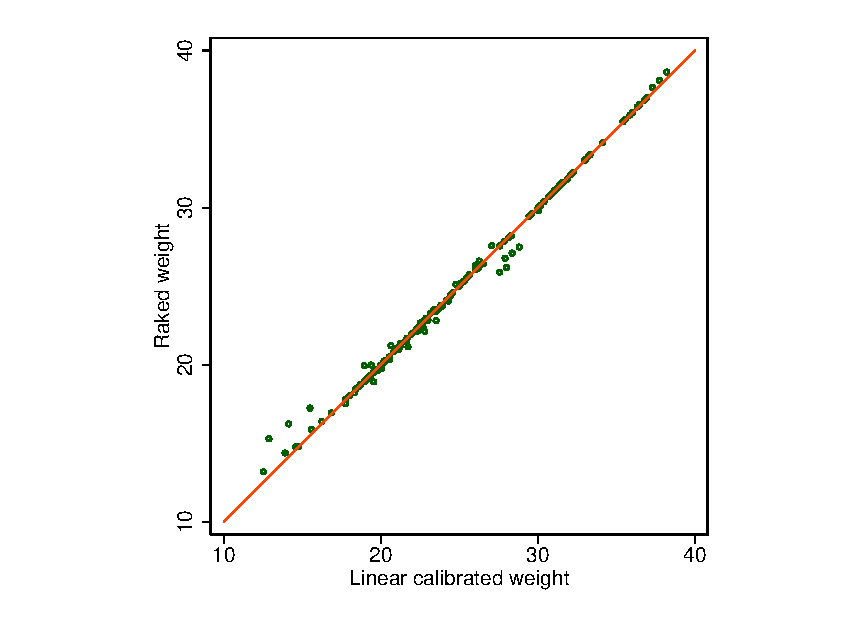
\epsfig{file=raked_linear,width=320}
    \end{center}
    \caption{Linear and raked weights}
    \label{fig:linear:raked}
\end{figure}

\clearpage

The speed advantages of \stcmd{linear} calibration are quite clear (0.63 seconds vs. 2.16 seconds),
even though raking convergence in 8 iterations is quite fast, in the author's experience
(it is not unusual to see dozens and hundreds of iterations, especially when higher order
interactions with many cells and subtle correlations between them are being used as
raking margins).
% TODO: time/profile better -- most of the time is spent in parsing
Linear calibrated and raked weights are very similar to one another, as Figure \ref{fig:linear:raked}
demonstrates, albeit the lowest of the linearly
calibrated weights are slightly smaller than comparable raked weights.
As the two methods are distinct, the weights should be expected to agree in general,
but the match along the diagonal line of the plot should not be expected to be ideal.

As mentioned before, in the extreme situations, linearly calibrated weights
may become negative, which creates additional issues.  First, Stata's \stcmd{svy}
commands or estimation commands with \stcmd{pweight} specifications do not accept
negative weights, and produce error messages when such weights are encountered.
(This is not a bug, but indeed a welcome behavior.) Second, negative weights are
typically difficult to interpret; within a common, although not technically accurate,
interpretation of sampling weights as the number of population units that a sampled
unit represents, it is puzzling to find a negative number of such population units.
The way the author uses the linear calibration functionality of \stcmd{ipfraking}
is to produce ``preliminary'' sets of weights. If the weights at the low end
satisfy the natural range restriction (greater than 0, so as not to produce
input data check errors with estimation commands; or sometimes greater than 1,
so as to satisfy the ``number of population units'' interpretation that is often
desirable for the clinets), these weights can be ``accepted'' as final. If they do not,
\stcmd{ipfraking} can be called with trimming syntax such as \stcmd{trimloabs(1)}.
The linear weights can then be used as a starting point to accelerate convergence.

% TODO: create an example where this is an issue, show the workaround
% See if this is internalized properly by svy calibrate linear.

While the general theory of calibrated estimation \citep{deville:sarndal:1992}
ensures that linear calibrated weights (analyzed as Case 1 in that paper) and
raked weights (Case 2) are asymptotically equivalent, this equivalence implicitly
requires that the scales of the population control matrices are identical.
In practice, different control total variables may come from different sources,
and some sources may have either different populations to which they can technically
be generalized, or come at different scales such as proportions vs. population totals.
Nearly every general population dual frame RDD survey that the present author had dealt
with would use the American Community Survey data for demographic variables
(that would come with the desirable population scaling), and National Health Interview Survey
data for phone use variables (cell phone only, landline only, both, or none) that would
come in the form of proportions. While the raking version of \stcmd{ipfraking} would not
have any difficulty incorporating both (with the caveat that the final scale of weights
will be determined by the \textit{last} variable in the \stcmd{ctotal()} list),
the linear version of weights would try to find a middle point between the population
totals that are on the scale of millions, and proportions that are on the scale of about 1.
The results would likely be quite strange.















\section*{Acknowledgements}

The author is grateful
to the anonymous referee for a thorough review and thoughtful suggestions,
to Tom Guterbock for bug reports and functionality suggestions,
and to Jason Brinkley for extensive comments and critique.
The opinions stated in this paper
are of the author only, and do not represent the position of Abt Associates.

\bibliographystyle{sj}
\bibliography{everything}
% \bibliography{ipfraking}

\begin{aboutauthor}
  Stanislav (Stas) Kolenikov is a Principal Scientist at Abt Associates.
  His work involves applications of statistical methods in data collection
  for public opinion research, public health, transportation, and other disciplines
  that utilize collection of survey data.
  Within survey methodology, his expertise includes advanced sampling techniques,
  survey weighting, calibration, missing data imputation, variance estimation,
  nonresponse analysis and adjustment, small area estimation, and mode effects.
  Besides survey statistics, Stas has extensive experience developing and applying
  statistical methods in social sciences, with focus on structural equation
  modeling and microeconometrics. He has been writing Stata programs since
  1998 when Stata was version 5.
\end{aboutauthor}
